\documentclass[thesis]{deutez}
\usepackage{amsmath}
\usepackage{graphicx}
\usepackage{caption}
\usepackage{pdfpages}
\usepackage{lscape}
\usepackage{rotating}
\usepackage{amssymb}
\usepackage{steinmetz}
\usepackage{xpatch}
\usepackage{esint}
\usepackage{gensymb}
\usepackage{mathtools}
\usepackage{xspace} 
%\usepackage{background}
\usepackage{comment}
\usepackage{bm}
\usepackage{physics}
%\usepackage{txfonts}
\usepackage{circuitikz}



\watermarklogo{Deu.jpg}  % Dokuz Eylül Üniversitesi Logosu; Sayfaya arkasına varsayılan logo olarak basılır.
%\projectname{DESIGN AND SIMULATION OF HIGH SPEED ELECTRO-OPTIC MODULATORS IN THIN-FILM LITHIUM NIOBATE ON INSULATOR PLATFORM}%
\projectname{Efficient and High Speed Electro-Optic Modulators In Thin Film Lithium Niobate}
\ogrencininadi{Efe KIRAZ}%
%\title{Research Project}
%\author{kiraz.efe }
%\time{03.06.2025}
\advisor{Dr. rer. nat. Reinhard Geiß\\ Dr. rer. nat. habil. Frank Setzpfandt}
%\jurya{Dr. rer. nat. Reinhard Geiß} % Replace with jury member names
%\juryb{Dr. rer. nat. habil. Frank Setzpfandt}
%\chair{Prof. Department Chair}

\begin{document}

    \begin{abstract}
        In this work, low-drive voltage based properties of electro-optic Mach Zehnder Modulator on thin film lithium niobate-on-insulator (LNOI) is analyzed through series of simulations in COMSOL6.0 multiphysics tool. First, the theory behind this cutting-edge modulator type is investigated with the help of well-known papers. Then $V_\pi L$ value of x-cut and z-cut LNOI is compared with previous work in literature in order to verify simulation method and physics used. Throughout simulations, optical wave and DC field distribution is analyzed and overlap integral between them is calculated by using MATLAB-COMSOL Livelink. After that, parametric sweeps was carried out to investigate how $V_\pi L$ value changes based on the geometric change. However, these changes also triggered optical losses in metalic electrode and dielectric interface. Metallic electrodes became mo Sweep parameter and loss change dependence is also investigated to see outcomes of geometrical changes. Eventually, excess amount of loss in z-cut modulators was drastically affected from top silica layer thickness and advantages of x-cut modulator was observed.
    \end{abstract}

\tableofcontents
\listoftables
\listoffigures

%\maketitle

\start

\chapter{INTRODUCTION}

    The needs of today's high-technology and science applications is determined by data manipulation capability at high rates. In order to supply this demand, new technologies are discovered which possesses transmission mechanism with low loss and data handling abilities at high bandwidth. 

    Electro-optic modulators are the backbone of today's data transmission systems owing to increasing data transfer rates. These building blocks make the most of relatively easy manipulation methods of electronics domain and low loss data transmission capability of optical domain at high bandwidth. In these devices, the light is modulated by externally applied electric field, at frequencies of radio, microwave or even terahertz. That modulation signal can be possibly generated by complementary metal-oxide-semiconductor (CMOS) electronics, which has very well defined manufacturing processes. 
   
% Having a widely-adopted CMOS signal levels makes easier integration of electronic and photonic system parts.

    Electro-optical modulation can be based on different phenomena for instance 
    quadratic electro-optic effect (Kerr effect) \cite{4}, Franz–Keldysh effect \cite{5}, quantum confined stark effect \cite{5}, free-carrier plasma dispersion effect \cite{3}. In this work, the focus of attention is on Pockels Effect due to advantages of high modulation speed and low insertion loss \cite{5}. Pockels effect is basically change of refractive index in propotion with applied electric field in non-centrosymmetric material. 
     
    An electrooptic material is expected to have low propagation loss, agile and low-loss optical modulation, efficient optical nonlinearity. There are several options in terms of the medium where electro-optic effects take place, for instance silicone (Si) \cite{6}, indium phosphide (InP) \cite{7}, silicone nitride (SiN$_x$), galleium arsenide(GaAs), alimunium nitride (AlN) and silicone carbide (SiC). Nevertheless, LiNbO$_3$ (LN) provides these properties in a relatively favorable way such as high $\chi^2$ nonlinearity, high Pockel's effect, high refractive index and wide transparency window \cite{1}. 
    
    \newpage
    
    Some of the important characteristic values for LiNbO$_3$ is seen in Table \ref{tab:ln_characteristics}
    
    

    \begin{table}[h]
        \centering
        \begin{tabular}{c|c|c|c|c|c|c}
            $r_{13}$ & $r_{51}$ & $r_{33}$ & $r_{22}$ & $n_o$ & $n_e$ & Transparency Window \\ \hline
            8.6 pm/V & 28 pm/V & 30.8 pm/V & 3.4 pm/V& 2.2111 & 2.1375 & 340$nm$ - 4.6$\mu m$
        \end{tabular}
        \caption{Characteristic values for LiNbO$_3$ at 1550nm wavelength \cite{8}}
        \label{tab:ln_characteristics}
    \end{table}
    
    where $r_{\#\#}$ represents the linear electro-optic tensor elements and $n_o$ and $n_e$ represents ordinary and extraordinary refractive indices, respectively. Due to 3m crystal symmetry of LN, some of the electro-optic tensor elements are zero. As it is seen on Table \ref{tab:ln_characteristics}, $r_{33}$ is largest electro-optic tensor element, taking role at change of index in Z crystal axis, and choosing x-cut LN crystal can provide advantageous in index manipulation with lower electric field amplitude. Moreover, large transparency window makes LN suitable for ultraviolet and mid-infrared applications.
   
    In the Table \ref{tab:losses_compared}, the typical loss values for several materials is seen. LN has considerably low optical insertion loss with respect to InP and other silicon photonics materials. 
    
    \begin{table}[h]
        \centering
        \begin{tabular}{|l|l|l|ll}
            \cline{1-2}
            Material Name & Loss (dB/cm) \\ \cline{1-2}
            InP \& SiPh & $>$1       \\ \cline{1-2}
            LN & 0.1-0.01     \\ \cline{1-2}
            SiN         & 0.01      \\ \cline{1-2}
        \end{tabular}
        \caption{Loss values for different materials\cite{9}}
        \label{tab:losses_compared}
    \end{table}
	
	These characteristics lead LN to find a place in numerous systems for instance on-space\cite{9}, radars\cite{23}, terahertz science \cite{22}. In these systems, TFLN based photonic integrated circuit (PIC) components are MZI based EO modulators, spiral bragg grating EO modulators, resonators and many more \cite{1}. Specifically, this master thesis is about Mach Zehnder Interferometer (MZI) modulator on thin-film LN-on-insulator (TFLNOI). 
	
	Capability of EO modulators is basically manipulation of properties of light for instance amplitude, phase, frequency, polarization, spatial or temporal behavior. By altering modulating signal or introducing different modulator networks input optical field properties are manipulated \cite{29}.
	
	MZI modulators can be driven by electrical signal, or modulating field, propagating through metallic planar electrodes or coplanar waveguides (CPWs). Since light is spatially modulated, efficient modulation is achieved by maximizing the interaction of modulating field and optical field. However, this is limited by losses appearing on metal electrodes \cite{14} due to absorption of optical field. As for high speed modulation, electrical signal can either be DC signal or higher frequency microwave field. As modulation signal frequency rises, modulation process suffers from several phenomenon and operation speed is limited by them \cite{14}, also demonstrated in Section \ref{sec:modulation_bandwidth}. This master thesis focuses on ways to facilitate the bandwidth of efficient EO modulator by analysing velocity of microwave field and optical field, impedance mismatch source and load ends of CPW and also microwave losses on CPW.
	
	In order to achieve high efficient modulation, microwave field is brought as close as possible to optical wave confined in LN waveguide, taking into account also metallic absorption. By considering this, numerous applications are realized by micro-structuring metallic electrodes \cite{24}, \cite{26}, \cite{28} or introducing additional material with lower absorption to metal electrodes  \cite{25}, \cite{27}
	
	In this master thesis, the main focus will be on micro-structuring of metalic electrodes due to in-house production capabilities of Fraunhofer IOF and needs of our research group. Eventually, intention of all the methods is to reduce current density travelling at the edges of coplanar waveguide so that loss decreases. 
	
	To sum up, achieving efficient and high speed modulator design nececitates efficient interaction of two fields, velocity and microwave impedance matching. In order to push the boundary of what is achieved, microwave losses has to be engineered.      
        
\chapter{THEORY}

    This section is primarily concerned about fundamental theory which explains how linear electro-optic phenomena works. Then, theoretical equipment to analyze MZI EO modulator will be introduced. Finally, phase and amplitude modulators will be discussed.

    \section{Maxwell's Equations}

    Mathematical model for propagation of electromagnetic wave (EMW) in vacuum is provided by Maxwell's equations as in the following,


    \begin{subequations}\label{eq:maxwell_def}
        \begin{align}
            \nabla \times \mathbf{E} &= -j\omega \mathbf{B} \label{eq:maxwell_def_a} \\
            \nabla \times \mathbf{H} &= \mathbf{J} + j\omega \mathbf{D} \label{eq:maxwell_def_b} \\
            \nabla \cdot \mathbf{D} &= \rho \label{eq:maxwell_def_c} \\
            \nabla \cdot \mathbf{B} &= 0 \label{eq:maxwell_def_d}
        \end{align}
    \end{subequations}

    % In the charge free medium, $\mathbf{J}$ and $\rho$ are equal to zero.
    Here $\mathbf{E}$ and $\mathbf{H}$ is the electric and magnetic field vectors, respectively. $\mathbf{D}$ and $\mathbf{B}$ correspond to electric and magnetic flux densities. $\mathbf{J}$ is current density vector and $\rho$ is charge density, which are source of the EMW. Also, constitutive relations define relation between field vectors with their corresponding flux densities and polarization effect of the medium.  

    \begin{align}
        \mathbf{D} &= \varepsilon_0 \mathbf{E} + \mathbf{P} = \varepsilon_0 \mathbf{E} + \varepsilon_0 \chi \mathbf{E} = \bm{\varepsilon} \mathbf{E} \label{eq:el_constitutive_def}\\
        \mathbf{B} &= \mu_0  \mathbf{H} + \mathbf{M}
       \label{eq:mag_constitutive_def} 
    \end{align}

    %$(\mathbf{r},\omega)$
    
    where $\varepsilon_0$ and $\mu_0$ are vacuum dielectric permittivity and permeability, $\chi$ is electrical susceptiblity, $\bm{\varepsilon}$ is relative permittivity tensor, $\mathbf{P}$ is induced electric polarizability and $\mathbf{M}$ is induced magnetic polarizability. Since this master thesis does not concern with magnetic mediums, induced magnetic polarizability is basically omitted in Equation (\ref{eq:mag_constitutive_def}). Furthermore, materials under analysis has the following properties: homogenenous, electrically isotropic and anisotropic, and non-magnetic.    
    
    \section{Transversal Field's Eigenvalue Equation}
    %\ref{sec:eigen-val-equation}

    Wave equation determines dispersion behavior in addition of electric and magnetic fields propagating in optical waveguide, they overall determine the mode characteristic. It is derived by using Equation (\ref{eq:maxwell_def}) under charge free medium condition. Ansatz for the guided modes are, 

    \begin{subequations}\label{eq:eigenval_eq}
        \begin{align}
            \mathbf{E}(x,y,z,\omega) &= \mathbf{E}(x,y,\omega)e^{-i\beta(\omega)z} \label{eq:ansatz_e} \\
            \mathbf{H}(x,y,z,\omega) &= \mathbf{H}(x,y,\omega)e^{-i\beta(\omega)z} \label{eq:ansatz_h}  
        \end{align}
    \end{subequations}
    
    In order to have eigenvalue equation for transverse fields, transversal and longitudinal components has to be splitted such that

    \begin{subequations}\label{eq:trans-longi_splitting}
        \begin{align}
            \mathbf{E}(x,y) &= \mathbf{E_{\perp}} + \mathbf{e}_z E_z(x,y) \label{eq:splitting_e} \\
            \mathbf{H}(x,y) &= \mathbf{H_{\perp}} + \mathbf{h}_z H_z(x,y) \label{eq:splitting_h} \\
             \mathbf{\nabla} &= \left( \nabla_{\perp}, \pdv{}{z} \right) 
        \end{align}
    \end{subequations}

    where $\nabla_{\perp} = (\pdv{}{x},\pdv{}{y}) $. First taking the curl of Equation (\ref{eq:maxwell_def_a}), 

    \begin{equation}
        \nabla \times (\nabla \times \mathbf{E}) = -j\omega \mu_0  (\nabla \times \mathbf{H})
        \label{eq:helmholtz1}
    \end{equation}

    by using the vector identity $\nabla \times (\nabla \times \mathbf{E}) = \nabla(\nabla \cdot \mathbf{E}) - \nabla^2 \mathbf{E}$ Equation (\ref{eq:helmholtz1}) becomes 

    \begin{equation}
        \nabla(\nabla \cdot \mathbf{E}) - \nabla^2 \mathbf{E} = -j\omega\mu_0 (\nabla \times \mathbf{H})
        \label{eq:helmholtz_vector_identity}
    \end{equation}

    considering charge free medium, we have $\nabla \cdot \mathbf{E}=0$ and $\mathbf{J}=\underline{0}$. Also substitute Equation (\ref{eq:maxwell_def_b}) into  Equation (\ref{eq:helmholtz_vector_identity}) by considering  Equation (\ref{eq:el_constitutive_def}),

    \begin{equation}
        - \nabla^2 \mathbf{E} = -j\omega\mu_0 (\nabla \times \mathbf{H})
        \label{eq:nebilimaq}
    \end{equation}
    
    Substitute Equation (\ref{eq:maxwell_def_b}) into right-hand side of Equation (\ref{eq:nebilimaq}),

    \begin{equation}
        \nabla_{\perp}^2 \mathbf{E}_{\perp} + \frac{\omega^2}{c^2}\bm{\varepsilon}(x,y) \mathbf{E}_{\perp} + \nabla_{\perp} (\mathbf{E}_{\perp} \nabla_{\perp} \ln(\bm{\varepsilon}(x,y)) ) = \beta^2 \mathbf{E}_{\perp}
        \label{eq:tranversal_eigenval}
    \end{equation}
    
    where $k(\omega)$ is wave number and defined as $\sqrt{\frac{\omega^2}{c^2}\bm{\varepsilon}(\mathbf{r},\omega)}$. Equation (\ref{eq:tranversal_eigenval}) is eigenvalue equation for the transversal components of the E-field in the medium which conceptually seen in Figure \ref{fig:2dWGgeom}. 
    
    
    \newpage
    In Equation (\ref{eq:tranversal_eigenval}) for the sake of simplicity, assumption of predominantly TE/TM polarized wave is propagating thorugh waveguide is made and fields become independent linearly polarized. Then, Equation (\ref{eq:tranversal_eigenval}) becomes,

    \begin{equation}
        \nabla_{\perp}^2 \psi + \frac{\omega^2}{c^2}\bm{\varepsilon}(x,y) \psi - \beta^2  \psi = 0
        \label{eq:tranversal_eigenval_scalar}
    \end{equation}

    where $\psi$ represents $E_x^{op}$ and $E_y^{op}$. 
    
    \begin{figure}[h]
        \centering
        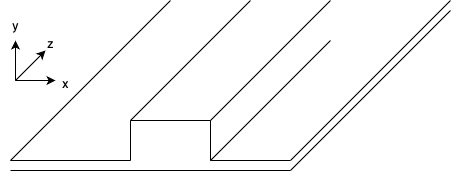
\includegraphics[width=0.5\linewidth]{2dWGgeom-2.png}
        \caption{Conceptual waveguide structure}
        \label{fig:2dWGgeom}
    \end{figure}
    
   
    
    \section{Electro-Optic Phenomena}
	\label{sec:electro-optic_phenomena}	
	
    This section consists of subtopics related with nonlinear susceptibility and index contraction, linear electro-optic effect (Pockels effect), index ellipsoid and its modulation. 

    \subsection{Nonlinear Polarization and Index Contraction}

     As a rule of thumb, susceptibility determines the relation between applied electric field and medium's response as it is seen in Equation (\ref{eq:el_constitutive_def}). Polarization can be expanded into its nonlinear terms, which represents more precisely the contributions of higher order terms such that

    \begin{equation}
        \mathbf{P} = \varepsilon_0 \left[ \bm\chi^{(1)} \mathbf{E}+\bm\chi^{(2)}\mathbf{E}^{2} +\bm\chi^{(3)}\mathbf{E}^{3} \dots  \right]
        \label{eq:pol_lin_nonlin}
    \end{equation}
    
    however, expansion of higher orders until the second term is sufficient since Pockel's effect is based on $\chi^{(2)}$ term.

    \begin{equation}
        \mathbf{P}(\mathbf{r},t) = \varepsilon_0 \bm\chi \overset{t}{\ast} \mathbf{E}(\mathbf{r},t)
        \label{eq:pol_def}
    \end{equation}

    In Equation (\ref{eq:pol_def}), symbol $\overset{t}{\ast}$ represents time convolution, which is explicitly

    \begin{equation}
        \begin{split}
        P_j(\mathbf{r},t) = \varepsilon_0 \sum_{k=x,y,z}\int_{-\infty}^{+\infty} \chi_{ik}(\mathbf{r},t-\tau)d\tau E_k(\mathbf{r},\tau) + \\ 
        + \varepsilon_0 \sum_{k=x,y,z}\sum_{l=x,y,z}\int_{-\infty}^{+\infty} \int_{-\infty}^{+\infty} \chi_{ikl}^{(2)}(\mathbf{r},t-\tau_1,t-\tau_2) E_k(\mathbf{r},\tau_1) E_l(\mathbf{r},\tau_2) d\tau_1 d\tau_2 
        \label{eq:pol_conv_explicit}
        \end{split}
    \end{equation}
    
    where $t-\tau<0$ (or $\tau_1$, $\tau_2$)  indicates causality of E-field and material interaction. $P_j(\mathbf{r},t)$ subindex indicates summation of E$-{field}$ contributions in three dimensions,  $\chi_{jkl}^{(2)}$ represents second order nonlinear susceptibility of the medium.

    In three dimensional case, $\mathbf{P}$ and $\mathbf{E}$ are vectors and susceptibility becomes tensor of third rank, linking one vector to the product of two others \cite{11}. For the sake of simplicity in calculations, E-field, $\mathcal{E} \cos(\omega t -\phi)$ in time domain, is represented in frequency domain as,

    \begin{equation}
        E = E(\omega_n) e^{-i\omega t} + E^*(\omega_{-n}) e^{i\omega t}
        \label{eq:e-field_freq}
    \end{equation}

    where $E(\omega)$ is complex amplitude and equal to $\frac{1}{2}\mathcal{E}e^{i \phi}$, where $\mathcal{E}$ is real amplitude and $\phi$ is phase. $\frac{1}{2}$ appears because physical field amplitude is divided between positive and negative frequency terms. It can be seen in Equation (\ref{eq:complex-identity}).
     
    \begin{equation}
        E^*(\omega) = \frac{1}{2}\mathcal{E}e^{i\phi}=E(-\omega)
        \label{eq:complex-identity}
    \end{equation}
    
    Similarly, second order polarization term is represented for one dimension in frequency domain is 

    \begin{equation}
        P^{(2)} = \sum_{n=\pm1} \sum_{m=\pm2} \chi^{(2)}(\omega_n,\omega_m)E(\omega_n)E(\omega_m)e^{-i(\omega_n+\omega_m) t}
        \label{eq:nonpol_freq}
    \end{equation}
    
    where susceptibility ($\chi$) is
    
    \begin{equation}
        \chi^{(2)} (\omega_n,\omega_m) = - \mathcal{N} \chi^{(1)} (\omega_n) \chi^{(1)} (\omega_m) \chi^{(1)} (\omega_n+\omega_m)
        \label{eq:chi_decomposition}
    \end{equation}
       
    where $\mathcal{N}$ is a constant depending on parameters in Lorentz model with anharmonic term. Second order $\chi^{(2)}$ is multiplication of first order susceptibilities for different frequency combinations and $\chi^{(1)}$ is real when polarization frequencies are far from resonance frequency of material's constituent atoms.  

    As for three dimensional nonlinear polarization in frequency domain, it becomes

    \begin{equation}
        P_i^{(2)} = \sum_{jk}\sum_{nm} \chi^{(2)}_{ijk}(\omega_n+\omega_m, \omega_n, \omega_m) E_j(\omega_n)E_k(\omega_m)e^{-i(\omega_n+\omega_m)t}
        \label{eq:sca_pol_conv_freq}
    \end{equation}

    where i,j,k each corresponds to cartesian axis x,y,z. Since $\chi^{(2)}$ is real then
    
    \begin{equation}
        \chi^{(2)}_{ijk}(\omega_n+\omega_m,\omega_n,\omega_m) = \chi^{(2)}_{ijk}(-\omega_n-\omega_m,-\omega_n,-\omega_m,)
        \label{eq:chi-real-condi}
    \end{equation}
    
    However, there are still 81 different independent nonlinear susceptibilities.  According to Equation (\ref{eq:chi_decomposition}) it is possible to reduce the number of nonlinear susceptibility terms such that,
    
    \begin{equation}
        \chi^{(2)}_{ijk}(\omega_n+\omega_m,\omega_n,\omega_m) = \chi^{(2)}_{jki}(\omega_n,\omega_m,-\omega_n-\omega_m) = \chi^{(2)}_{kij}(\omega_m,\omega_m+\omega_n,\omega_n)
        \label{eq:index_reducation}
    \end{equation}

    this means subindices $i,j,k$ can be permuted with frequencies $n,m$. As a result, 81 different nonlinear susceptibilities are reduced to 27. Equation (\ref{eq:sca_pol_conv_freq}) can be written in terms of optical and electrical frequencies,

    \begin{equation}
        P_i^{(2)} = \sum_{jk}\sum_{nm} \chi^{(2)}_{ijk}(\omega^{opt}_n, \omega^{el}_m) E^{opt}_j(\omega^{opt}_n)E^{el}_k(\omega^{el}_m)e^{-i(\omega^{opt}_n+\omega^{el}_m)t}
        \label{eq:sca_pol_conv_freq_opt_el}
    \end{equation}

    The frequency term $(\omega_n+\omega_m)$ in $\chi^{(2)}_{ijk}$ is dropped because optical frequency are in the range of THz and microwave frequency is in GHz range. Summation of them will approximately equal to optical frequency. 
    
    One important rule which connects nonlinear susceptibility to nonlinear electro-optic constant $d$. When Equation (\ref{eq:chi_decomposition}) is generalized for three dimension,

    \begin{equation}
        \chi^{(2)}_{ijk} = \chi^{(1)}_{ii} (\omega_n) \chi^{(1)}_{jj} (\omega_m) \chi^{(1)}_{kk} (\omega_n+\omega_m) \Delta_{ijk}
        \label{eq:miller}
    \end{equation}

    Equation (\ref{eq:miller}) is called as Miller rule, who found the relation and stated that $\Delta_{ijk}$ is almost constant for many materials \cite{11}. The relation between nonlinear susceptibility or nonlinear electro-optic constant is 

    \begin{equation}
        d_{ijk} = \frac{1}{2}\chi^{(2)}_{ijk}
        \label{eq:sus-const}
    \end{equation}

    %In order to demonstrate interaction between optical field and microwave field in nonlinear medium, time convolution needs to be evaluated, by using Volterra series expansion. 

    % $E_k(\mathbf{r},t)$ represents optical electric field ($E^{opt}$) and $E_l(\mathbf{r},\tau_2)$ represents modulating electric field ($E^{el}$). Specifically, $\chi_{jkl}^{(2)}$ is responsible from Pockels effect, or linear electro-optic effect. 
    
    %In Eq [\ref{eq:pol_lin_nonlin}], which is frequency domain correspondance of Eq [\ref{eq:pol_conv_explicit}] implicitly, polarization is expanded into its linear term (containing $\bm\chi^{(1)}$) and nonlinear terms (higher orders of $\bm\chi^{(1)}$). In order to analyze nonlinearity, wave equation derivation is revisited, however, this time Eq [\ref{eq:maxwell_def_b}] and [\ref{eq:el_constitutive_def}] will be substituted into Eq [\ref{eq:nebilimaq}] without omitting polarization term because the purpose is to analyze nonlinearity of medium to the applied modulating field. Moreover, the first term in Eq [\ref{eq:helmholtz_vector_identity}] is not generally zero in nonlinear optics due to more general relation in Eq [\ref{eq:el_constitutive_def}]. Fortunately, the first term of Eq [\ref{eq:helmholtz_vector_identity}] is dropped for the cases of interest. Generally, slowly varying envelope approximation (SVEA) validates dropping that term in vector identity \cite{10} then based on this assumption, nonlinear equation is obtained as,

    %\begin{equation}
    %    \nabla^2 \mathbf{E} + \frac{\omega^2}{c^2} \bm \varepsilon \mathbf{E} = -\frac{\omega^2}{c^2} \mathbf{P^{NL}} = -\frac{\omega^2}{c^2} \bm\chi^{(2)} \mathbf{E^2}
    %    \label{eq:waveEqNonlinear}
    %\end{equation}

    %In order to explicitly demonstrate optical and RF field, modulating refractive index of nonlinear medium, Eq [\ref{eq:waveEqNonlinear}] is rearranged as,

    %\begin{equation}
    %    \nabla^2 \mathbf{E^{optical}} + \frac{\omega^2}{c^2} \bm \varepsilon \mathbf{E^{optical}} = -\frac{\omega^2}{c^2} \mathbf{P^{NL}} = -\frac{\omega^2}{c^2} \bm\chi^{(2)} \mathbf{E^2}
    %    \label{eq:waveEqNonlinear_explicit}
    %\end{equation}

    %   As it can be seen in Eq \ref{eq:second-order-pol}, second order process generates a new third frequency component at $\omega_3$. As a result, $\chi^{2}$ can be written as, 
    % and $E_2 = E^0_2\cos(\omega_2t+kz)$
    %\begin{equation}
    %    \chi^{2} = \chi^{2}(\omega_3,\omega_2,\omega_1)
    %    \label{eq:chi}
    %\end{equation}

    %When two waves, having $\omega_1$ and $\omega_2$ frequencies, interact in such medium, it is convenient to analyze the content of second order polarization term $P^{(2)}$. 

    %\begin{equation}
    %    P^{(2)} = P_0 + P_{\omega_1+\omega_2} + P_{\omega_1-\omega_2} + P_{2\omega_i}
    %    \label{eq:second-order-pol}
    %\end{equation}
    
    %where $P_0$ is called as DC polarizarion, $P_{\omega_1 \pm \omega_2}$ is mixed form and $P_{2\omega_i}$ is second harmonic -where $i$ is 1 or 2. Special case is second harmonic generation where $\bm\chi^{(2)} = \bm\chi^{(2)}(2\omega,\omega,\omega)$. Assume the interacting wave are $E = E^0\cos(\omega t+kz)$.  In order to simplify derivation $d$ is defined such that $ d = \varepsilon_0 \bm \chi^{(2)}$. Then the terms in Eq[\ref{eq:second-order-pol}] become

    %\begin{subequations}\label{eq:second-order-pol-detail}
    %   \begin{align}
    %        P_0 &= 2d (E^0)^2 \label{eq:fund-dc} \\
    %       P_{\omega_1-\omega_2} &= d(E^0)^2 \label{eq:difference-freq} \\
    %       P_{\omega_1+\omega_2} = P_{2\omega} &= d(E^0)^2\cos(2\omega t + 2kz) \label{eq:sum-freq} 
    %   \end{align}
    %\end{subequations}
    
    %Eq[\ref{eq:second-order-pol-detail}] is basically obtained by using commutativity of electric field multiplications. This indicates 

    %\begin{equation}
    %    P^{(2\omega)}_i = d_{ijk} E_jE_k = d_{ikj} E_kE_j
    %    \label{eq:index-contraction}
    %\end{equation}

    %where $d_{ijk}$ is $3\times 3 \times 3$ matrix.
    
    \subsubsection{Index Contraction}

    There is no noticeable physical correspondence to compare precedence of modulating electrical field over optical field, or vice versa. Derivations did not consider this order mathematically up to now. Here definition of column vector $F$ indicates insignificance of multiplication order. One element of $F$ is defined such that

    \begin{equation}
        F_l = (1-\frac{1}{2}\delta_{jk})(E_j(\omega_{opt})E_k(\omega_{el})+E_k(\omega_{el})E_j(\omega_{opt}))
        \label{eq:F}
    \end{equation}

    where $\delta$ indicates Kronecker symbol and is defined as $\delta_{jk}=1$ when $j=k$. Then $\mathbf{F}$ is 

    \begin{equation}
    \mathbf{F=}
    \begin{bmatrix}
        E_x(\omega_{opt})E_x(\omega_{el}) \\
        E_y(\omega_{opt})E_y(\omega_{el}) \\
        E_z(\omega_{opt})E_z(\omega_{el}) \\
        E_y(\omega_{el})E_z(\omega_{opt})+E_z(\omega_{el})E_y(\omega_{opt}) \\
        E_x(\omega_{el})E_z(\omega_{opt})+E_z(\omega_{el})E_x(\omega_{opt}) \\
        E_x(\omega_{el})E_y(\omega_{opt})+E_y(\omega_{el})E_x(\omega_{opt})
    \end{bmatrix}
    \label{eq:F_matrix}
    \end{equation}

    
    
    The Table \ref{tab:index-contraction} shows how the index is contracted

    \begin{table}[h]
        \centering
        \begin{tabular}{|c|c|c|c}
            \cline{1-2}
            $jk$ & $l$ \\ \cline{1-2}
            xx   & 1       \\ \cline{1-2}
            yy   & 2     \\ \cline{1-2}
            zz   & 3    \\ \cline{1-2}
            yz/zy   & 4    \\ \cline{1-2}
            xz/zx   & 5    \\ \cline{1-2}
            xy/yx   & 6    \\ \cline{1-2}
        \end{tabular}
        \caption{Index contraction providing $d_{ijk} \rightarrow d_{il}$ transition}
        \label{tab:index-contraction}
    \end{table}

    Polarization and $\mathbf{F} $ is related such that

    \begin{equation}
        P_i = 2d_{il} F_l
        \label{eq:pol-with-F}
    \end{equation}
    
    where d is defined previously in Equation (\ref{eq:sus-const}). As a result, the number of elements in 2$^{nd}$ order susceptibility tensor is reduced from 27 elements to 18 elements.  Matrix form of Equation (\ref{eq:pol-with-F}) is seen below,

    \begin{equation}
    \begin{bmatrix}
        P_x \\
        P_y \\
        P_z 
    \end{bmatrix}
    =
    \begin{bmatrix}
        d_{11} \; d_{12} \; d_{13} \; d_{14} \; d_{15} \; d_{16} \\
        d_{21} \; d_{22} \; d_{23} \; d_{24} \; d_{25} \; d_{26} \\
        d_{31} \; d_{32} \; d_{33} \; d_{34} \; d_{35} \; d_{36} \\
    \end{bmatrix}
    \begin{bmatrix}
        E_x(\omega_{opt})E_x(\omega_{el}) \\
        E_y(\omega_{opt})E_y(\omega_{el}) \\
        E_z(\omega_{opt})E_z(\omega_{el}) \\
        E_y(\omega_{el})E_z(\omega_{opt})+E_z(\omega_{el})E_y(\omega_{opt}) \\
        E_x(\omega_{el})E_z(\omega_{opt})+E_z(\omega_{el})E_x(\omega_{opt}) \\
        E_x(\omega_{el})E_y(\omega_{opt})+E_y(\omega_{el})E_x(\omega_{opt})
    \end{bmatrix}
    \label{eq:F_matrix_equation}
    \end{equation}

    \subsection{Linear Electro-Optic Effect and Index Ellipsoid}
    
    The phenomena is also known as Pockels effect, it is linear relation between applied electric field and change of refractive index. Basically, Pockels medium can alter the phase of EM wave by means of induced birefringence when polarizing electric field is applied to the medium, or Pockels cell. Here, electric field which is polarizing the medium is different than the field desired to alter its phase. This condition is critical because it makes the distinction quadratic electro-optic (Kerr-Effect) from linear electro-optic effect.
    
    In an anisotropic medium, propagation of waves is direction dependent. This requires a wave vector $\mathbf{k}$ definition based on propagation direction. 
    
    \begin{equation}
        \mathbf{k} = n_s \frac{\omega}{c_0} \mathbf{s}
        \label{eq:direction-dependent-wave-vector}
    \end{equation}  
    
    where $n_s$ is defined as unknown refractive index which wave experience in its propagation direction which is defined by $\mathbf{s}$. $\frac{\omega}{c_0}$ corresponds to free space wave number for that frequency. By substituting ansatz for plane waves Equation (\ref{eq:ansatz_e}), Equation (\ref{eq:ansatz_h}) into Maxwell equations Equation (\ref{eq:maxwell_def}) and also considering constitutive relation Equation (\ref{eq:el_constitutive_def}) and Equation (\ref{eq:direction-dependent-wave-vector}), Fresnel equation is obtained to prove that different polarization of electric field $\mathbf{E}$ experience different refractive index.

    \begin{equation}
        \frac{s_x^2}{n_s^2 - n_x^2} + \frac{s_y^2}{n_s^2 - n_y^2} + \frac{s_z^2}{n_s^2 - n_z^2} = \frac{1}{n_s^2}
        \label{eq:fresnel-eq}
    \end{equation} 

    where $n_x$, $n_y$, $n_z$ is derived as $n_{ij}=\sqrt{\frac{\varepsilon_{ij}}{\varepsilon_0}}$, based on dielectric tensor $\bm\varepsilon$

    \begin{equation}
        \bm\varepsilon=\varepsilon_0
        \begin{bmatrix}
            \varepsilon_{xx} & 0 & 0\\
            0 & \varepsilon_{yy} & 0\\
            0 & 0 & \varepsilon_{zz}
        \end{bmatrix}
        =
        \begin{bmatrix}
            n^2_{x} & 0 & 0\\
            0 & n^2_{y} & 0\\
            0 & 0 & n^2_{z} 
        \end{bmatrix}
        =
        \begin{bmatrix}
            n^2_{o} & 0 & 0\\
            0 & n^2_{o} & 0\\
            0 & 0 & n^2_{e} 
        \end{bmatrix}
        \label{eq:dielectric-tensor}
    \end{equation}
    
    where $n_o$ indicates ordinary refractive index and $n_e$ is extraordinary refractive index. From this second order equation Equation (\ref{eq:fresnel-eq}), there will be linearly independent two linearly polarized electric flux density. They will be later used in index ellipsoid. For LN which belongs to class of negative uniaxial crystals, dielectric tensor components in each direction is related such that $\varepsilon_{zz} < \varepsilon_{xx}=\varepsilon_{yy}$. 

     
    According to Yariv and Pochi, propagation of electromagnetic wave in linear electro-optic medium is best described in terms of index ellipsoid \cite{2}. 

    \begin{equation}
        D_i = \varepsilon_{ij}E_j^{el}
        \label{eq:flux-den}
    \end{equation}

    The Equation (\ref{eq:constant-energy-surf}) defines constant energy density in $\mathbf{D}$-space. 
    
    \begin{equation}
        U_e = \frac{1}{2}\mathbf{D}.\mathbf{E} = \frac{1}{2} \mathbf{D} \varepsilon_0^{-1}(\bm\varepsilon^{-1}.\mathbf{D}) = \frac{1}{2\varepsilon_0} \left[ \frac{D_x^2}{\varepsilon_{xx}} + \frac{D_y^2}{\varepsilon_{yy}} + \frac{D_z^2}{\varepsilon_{zz}} \right]
        \label{eq:constant-energy-surf} 
    \end{equation}

    where $\varepsilon_{ii}$ ($i=x,y,z$) are defined in Equation (\ref{eq:dielectric-tensor}). 

    In order to define principle indices of refraction, the relation $\mathbf{r}=\frac{\mathbf{D}}{\sqrt{2\varepsilon_0U_e}}$ is defined. Then index ellipsoid can be written such that,

    \begin{equation}
        \frac{x^2}{n_x^2}+\frac{y^2}{n_y^2}+\frac{z^2}{n_z^2}=1
        \label{eq:index_ellipsoid}
    \end{equation}


    Equation (\ref{eq:index_ellipsoid}) is mainly used to determine electric flux density vectors and is demonstration of Fresnel equation Equation (\ref{eq:fresnel-eq}). Index ellipsoid and the plane, which is normal to the direction of propagation $\mathbf{s}$, intersects each other. This intersection has ellipse shape in anisotropic materials and axes of this ellipse has length of $2n_1$ and $2n_2$, indicating two orthogonal directions. 

    \begin{figure}[htbp]
        \centering
        \begin{minipage}{0.45\textwidth}
            \centering
            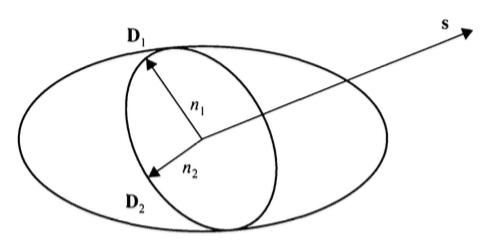
\includegraphics[width=\linewidth]{indexEllipsoidMethod.png}
            \vspace{0.3cm}
            \caption{Index ellipsoid method. The inner ellipse is the intersection of the index ellipsoid with the plane that is normal to $\mathbf{s}$ and passes through the center of the ellipsoid \cite{2}}
            \label{fig:left}
        \end{minipage}
        \hspace{1.5cm}
        \begin{minipage}{0.25\textwidth}
            \centering
            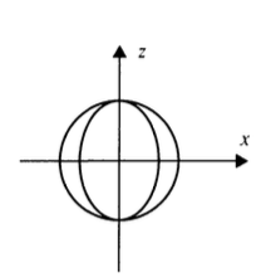
\includegraphics[width=1\linewidth]{negativeUniaxialCrystal.png}
            \caption{Negative uniaxial crystal normal surfaces, $n_o$ is in z-direction and $n_e$ is in x direction \cite{2} }
            \label{fig:right}
        \end{minipage}
    \end{figure}

    In Equation (\ref{eq:index_ellipsoid}), each $\frac{1}{n^2_{i}}$ $(i=1,2,3)$ corresponds to principle values of impermeability tensor, defined as

    \begin{equation}
        \eta = \frac{\varepsilon_0}{\varepsilon}
        \label{eq:impermeability}
    \end{equation}

    Application of electric field causes redistribution of charges in material and slight deformation in crystal structure. Net change is the change of impermeability tensor. 

    \begin{equation}
        \Delta\eta _ {ij} = \eta(\mathbf{E})-\eta(0) \equiv \Delta \left( \frac{1}{n^2} \right)_{ij} \equiv r_{ijk}E_k^{el}
        \label{eq:elect-opt-mod-imperm}
    \end{equation}

    where $E_k$ indicates modulating electric field in $x,y,z$-directions and $r_{ijk}$ corresponds to linear electro-optic coefficients. As for LN, it belongs to 3m crystal symmetry class, which leads to linear electro-optic tensor $r_{ij}$ in the form,

    \begin{equation}
        r_{ij}=
        \begin{bmatrix}
            0 & -r_{22} & r_{13}\\
            0 & r_{22} & r_{13} \\
            0 & 0 & r_{33}\\
            0 & r_{51} & 0\\
            r_{51} & 0 & 0\\
            -r_{22} & 0 & 0 
            
        \end{bmatrix}
        \label{eq:3m-linear-el-opt-tensor}
    \end{equation}

    and deformed index ellipsoid is,

    \begin{equation}
        \left(\frac{1}{n_o^2} + r_{13}E^{el}\right)x^2+\left(\frac{1}{n_o^2} + r_{13}E^{el}\right)y^2+\left(\frac{1}{n_e^2} + r_{33}E^{el}\right)z^2 = 1
        \label{eq:deformed-index-ellipsoid}
    \end{equation}
    
    having no mixed terms in Equation (\ref{eq:deformed-index-ellipsoid}) results in unchanged principle axis of modulated index ellipsoid. Lengths of axis in new index ellipsoid are in the form $n+\Delta n$ which is,

    \begin{subequations}\label{eq:index-ellipsoid-lengths}
    \begin{align}
        n_x = n_o- \frac{1}{2}n_o^3 r_{13}E^{el} \label{eq:index-ellipsoid-lengths-nx}\\ 
        n_y = n_o- \frac{1}{2}n_o^3 r_{13}E^{el} \label{eq:index-ellipsoid-lengths-ny}\\
        n_z = n_e- \frac{1}{2}n_e^3 r_{33}E^{el} \label{eq:index-ellipsoid-lengths-nz}
    \end{align}
    \end{subequations}

    The terms containing $E^{el}$ will be used to derive overlap integral in Section \ref{sec:el-op-fom}. If a light beam is propagating along $x$-direction then the refractive index it experiences is

    \begin{equation}
        n_z-n_y= (n_e-n_o)-\frac{1}{2}(n_e^3 r_{33}-n_o^3 r_{13})E^{el}
    \end{equation}
    
    \section{Optical Waveguide}
    %\ref{sec:optical-waveguides}
    
    Optical field is confined and propagates through this medium. During the propagation, optical field experiences modulated refractive index, that is to say, this is the medium where Pockles effect takes place. Early designs was consisting of titanium (Ti) diffused bulk LN waveguide. In this fabrication method, Ti-strip is diffused into host material bulk LN through thermal annealing and resulting medium satisfies weak guidance of optical wave in a relatively large optical mode area with respect to thin film (TF) applications. Large optical mode dictates also placement of microwave waveguides far away from optical modes, which is detrimental for overlap integral. Otherwise gold electrodes absorbs optical field based on plasmonic effects. As a result, having large mode area results in reduced overlap between RF and optical fields which leads to increase of $V_{\pi}.L$ values. 

    The ultimate aim is integrating EO modulators with a small footprint into CMOS electronic chips and this requires reduced drive voltages in optical waveguide sections \cite{14} \cite{15}. TFLNOI provides high optical field confinement so that RF and optical fields overlap and drive voltage decreases. This is one of the main reason to prefer thin-film-on-insulator structure other than bulky waveguides. 

    \begin{figure}[htbp]
        \centering
        \begin{minipage}{0.4\textwidth}
            \centering
            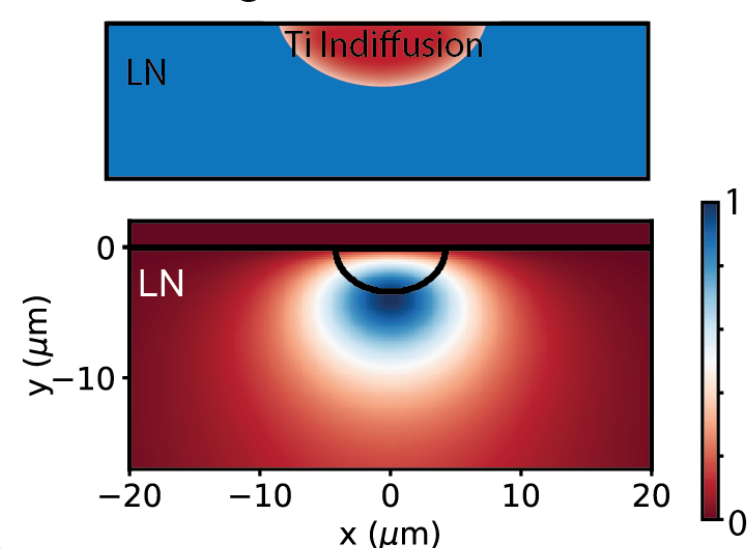
\includegraphics[width=\linewidth]{ion-diffused.png}
            
            \caption{Overlap area in ion diffused LN waveguide is more than 10 times larger with respect to monolithic-rib-ridge waveguide on the right  \cite{1}.}
            \label{fig:ion_diffused_LN_wg}
        \end{minipage}
        \hspace{1.5cm}
        \begin{minipage}{0.4\textwidth}
            \centering
            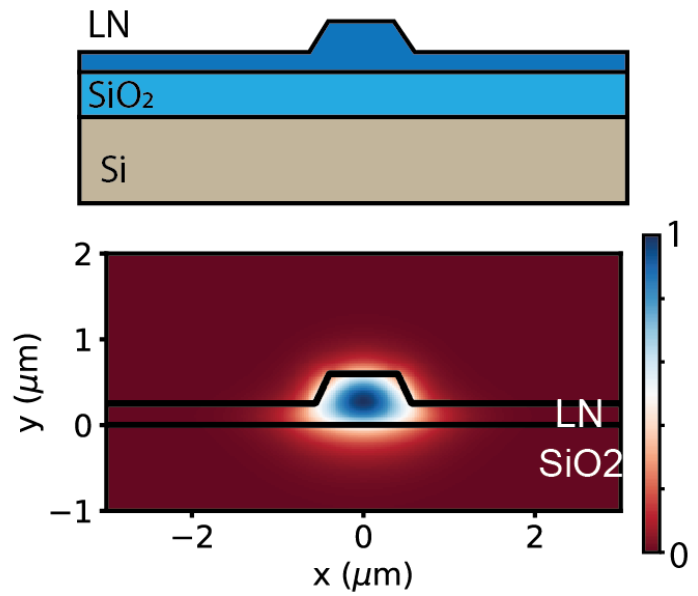
\includegraphics[width=1\linewidth]{monolithic-rid-ridge.png}
            \caption{Monolithic-rib-ridge waveguide consists of oxide layer and a substrate in addition to LN \cite{1}.}
            \label{fig:rib-ridge_LN_wg}
        \end{minipage}
    \end{figure}

    In reference to crystal axis of LN, the direction in which bulk material is cut determines which polarization of E-field experiences extraordinary refractive index. Taking into account this condition, placement of electrodes supposed to be oriented in a way such that polarization of RF electric field and optical electric field matches with optical axis of the crystal.

    \begin{figure}[h]
        \centering
        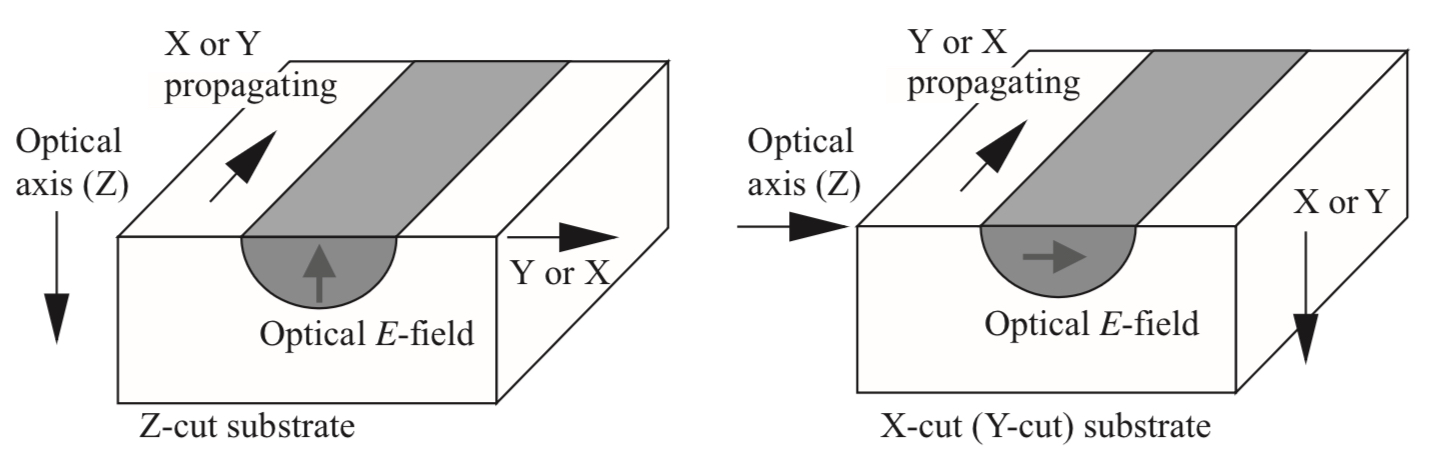
\includegraphics[width=0.8\linewidth]{modulator-orientation.jpeg}
        \caption{Cut direction in fabrication process determines modulator geometry\cite{16} (the same directional reference applies also thin-film waveguides)}
        \label{fig:waveguide-orientation}
    \end{figure}
    
    In Figure \ref{fig:waveguide-orientation} on the right, x-cut substrate is seen. In x-cut substrate, optical axis is in-plane of wafer surface. Optical field is through the optical axis of crystal. Corresponding mode polarization for optical electric field is TE-polarization. On the left, z-cut substrate is seen. This time optical field out-of-wafer-surface. This leads to different electrode placement. In Figure \ref{fig:electrode-placement}, microwave elctrode placement is seen. On the left, electrodes are alligned horizontally in x-cut crystal structure and vertically aligned electrodes are seen on the right.

    \begin{figure}
        \centering
        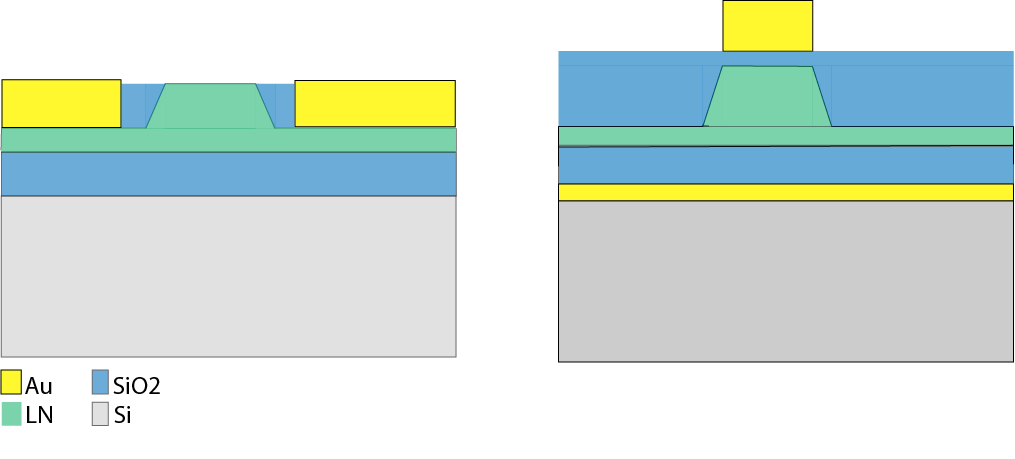
\includegraphics[width=0.9\linewidth]{x-cut-LNOI.png}
        \caption{Electrodes are placed depending on crystal-cut so that overlap of fields achieved. X-cut LN is on the left and Z-cut LN is on the right }
        \label{fig:electrode-placement}
    \end{figure}
 
    
    As for the application point of view, polarization maintaining fiber has to be utilized to ensure the polarization of the light shine onto integrated waveguide facet.

    \section{Coplanar Waveguide}
    \label{sec:coplanar_waveguide}

    Applied modulating field is in the range of GHz frequencies and this requires integration of microwave transmission line, or specifically coplanar waveguide. The wave has complex propagation constant,

    \begin{equation}
        \gamma_{el} = \alpha_{el} + j\beta_{el} = \alpha_{el} +j \frac{\omega}{c} n_{el}
        \label{eq:mic-prop-const}
    \end{equation}

    where $\gamma_{el}$ is complex microwave propagation constant, $\alpha_{el}$ [Np/m] is electrical losses and $\beta_{el}$ [rad/m] is phase constant of the line and $n_{el}$ microwave effective index.

    %Characteristic impedance for a lossy line is 

    %\begin{equation}
    %    Z_0 = \sqrt{\frac{R' + j\omega L'}{G' + j\omega C'}}
    %    \label{eq:lossy-char-eq}
    %\end{equation}

    %where R' $[\Omega/m]$, L'$[H/m]$, C'$[F/m]$, G'$[S/m]$ are combined resistance, inductance, capacitance and conductance of both conductors per unit length. 

    \begin{figure}[h]
        \centering
        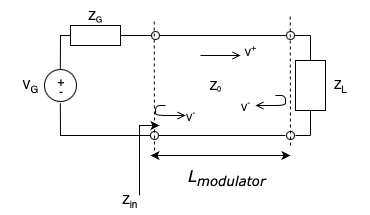
\includegraphics[width=0.5\linewidth]{TL_model.png}
        \caption{Generic microwave transmission line}
        \label{fig:transmissionline.png}
    \end{figure}

	In Figure \ref{fig:transmissionline.png}, $Z_0$ corresponds to characteristic impedance of the line. It is considered as figure of merit for a transmission line and it is based on unit length parameters of the line, given in Figure \ref{fig:lumped_model_of_transmission_line}. Characteristic impedance of lossy line is given as 
	
	\begin{equation}
		Z_0 = \sqrt{\frac{R+j\omega L}{G+j\omega C}}
		\label{eq:characteristic_impedance}	
	\end{equation}		

	

    Another important parameter for microwave transmission line is input impedance as seen from the input of the line in figure 
    \begin{equation}
        Z_\text{in} = Z_0 \frac{Z_L + Z_0 \tanh(\gamma_{el} l)}{Z_0 + Z_L \tanh(\gamma_{el} l)}
        \label{eq:input-impedance}
    \end{equation}

    where $Z_L$ is load impedance. Input impedance is depending on load, the electrical length and characteristic impedance of the transmission line .

    The wave travelling through coplanar waveguide is in quasi-TEM mode, which assumes longitudinal field components is small relative to transverse field components. Several design parameters exist for coplanar waveguides such that,
    
    \begin{enumerate}
        \item Trace width (S)
        \item Gap between signal and ground sections (w)
        \item Effective dielectric constant of substrate ($\varepsilon_{eff})$
        \item Thickness of dielectric (h)
    \end{enumerate} 

    \begin{figure}[h]
        \centering
        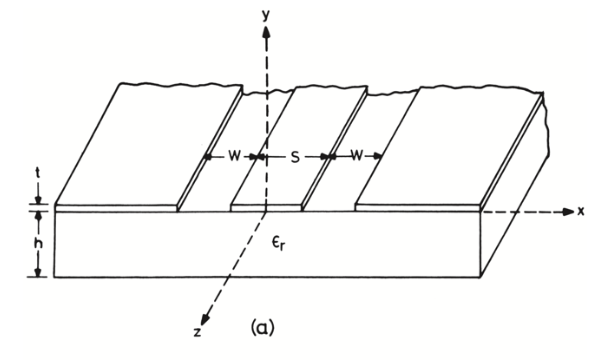
\includegraphics[width=0.6\linewidth]{cpw.png}
        \caption{Geometry of coplanar waveguide \cite{12}}
        \label{fig:cpw}
    \end{figure}
	
	As seen on Figure \ref{fig:electrode-placement}, multilayer structure consists of different materials which give rise to effective dielectric permittivity for microwave electric field, as opposed to Figure \ref{fig:cpw}.
	
    Lumped model of the line consists of equivalent resistance (R) and inductance of the line (L), line capacitance (C) and displacement field lossess (G) in dielectric. 

    


    \section{Mach Zehnder Electrooptic Modulator Types}

    Mach Zehnder modulators are based on interferometry phenomenon. In the context of this work, single electrode driving modulators are investigated. However, there are other types of driving applications which are called as dual electrode driving and two stage dual electrode driving in order to achieve more complex operations \cite{20}. 

    In the Figure \ref{fig:modulator} basic phase modulator is seen on the left, it consists of microwave strip line and one optical waveguide. As for the one on the right, it is responsible from intensity modulation and it consists of CPW, MZI with 50:50 Y-splitter.
 
    \begin{figure}[h]
        \centering
        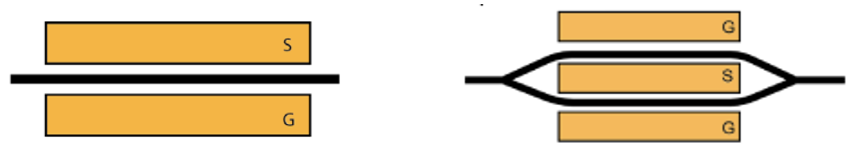
\includegraphics[width=0.8\linewidth]{Screenshot 2025-05-20 at 17.35.40.png}
        \caption{Phase modulator is seen on the left and MZI intensity modulator with upper and lower arms is on the right\cite{1}}
        \label{fig:modulator}
    \end{figure}

    Phase modulator is basic building block of intensity modulation. In intensity modulation it is based on constructive and destructive interference. Excitation of $V_\pi$ voltage causes 180$\degree$ phase shift between two arms which ends up having destructive interference and "OFF" state. When there is no excitation applied, both arms are in phase which corresponds to "ON" state.
    
    Static EO response starts with considering 3-port, matched, lossless Y-splitter with output ports are isolated. Following the notation in \cite{16}, scattering parameters of such structure is 

    \begin{equation}
        \bm{S_{sp}} =
        \begin{bmatrix}
            0 & \sqrt{\alpha}\,e^{j\phi_{sp}} & \sqrt{1-\alpha}\,e^{j\phi_{sp}}\\
            \sqrt{\alpha}\,e^{j\phi_{sp}} & 0 & 0 \\
            \sqrt{1-\alpha}\,e^{j\phi_{sp}} & 0 & 0\\
            
        \end{bmatrix}
        \label{eq:linear-el-opt-tensor}
    \end{equation}

    where $\alpha$ indicates power asymmetry for asymmetric splitter, for 50:50 splitter $\alpha=0.5$. This matrix satisfies losslessness condition, $\bm S_{sp}\bm S^\dagger_{sp} =1$. When its input power at port 1 is \textit{$a_1$}, output power at port 2 and port 3, 

    \begin{subequations}\label{eq:MZM-splitter-s-matrix}
        \begin{align}
             b_2 = \sqrt{\alpha}\,e^{j\phi_{sp}} a_1 \label{eq:MZM-splitter-s-matrix-b2} \\
             b_3 = \sqrt{1-\alpha}\,e^{j\phi_{sp}} a_1\label{eq:MZM-splitter-s-matrix-b3}
        \end{align}
    \end{subequations}
    
    Scattering matrix for combiner, with input ports \textit{$a'_2$} (upper arm) and \textit{$a'_3$} (lower arm), is the same with splitter. The assumption for perfectly matched upper and lower arms is made and combiner inputs are

    \begin{subequations}\label{eq:MZM-combiner-s-matrix}
        \begin{align}
             a'_2 = \sqrt{\alpha}\,e^{j\phi_{sp}} \,a_1\,e^{-jk_0L-j\Delta\phi_U} \label{eq:MZM-combiner-s-matrix-a2} \\
             a'_3 = \sqrt{1-\alpha}\,e^{j\phi_{sp}} \, a_1\, e^{-jk_0L-j\Delta\phi_L} \label{eq:MZM-combiner-s-matrix-a3}
        \end{align}
    \end{subequations}
    
    Then combiner output becomes

    \begin{equation}
        b'_1 = e^{2j\phi_{sp}}e^{-jk_0L} \left[ \alpha e^{-j\Delta\phi_U} + (1-\alpha) e^{-j\Delta\phi_L} \right] a_1
    \end{equation}

    Impedances are the same at the input and the output of the couplers, then 

    \begin{equation}
        T(V_{in}) = \frac{P_{out}}{P_{in}} = \left| \frac{b_1'}{a_1} \right|^2 = \eta \left\{ 1 + 2\alpha(1 - \alpha)\left[ \cos(\Delta\phi_U - \Delta\phi_L) - 1 \right] \right\}
    \end{equation}

    where $\eta$ represents optical insertion loss of the modulator. For the symmetrical case where $\alpha=0.5$, 

    \begin{equation}
        T(V_{in}) = \frac{\eta}{2} \left[ 1+\cos(\Delta\phi_U - \Delta\phi_L) \right] 
        \label{eq:transmission-char-equal-splitter} 
    \end{equation}

    Splitters are symmetric but upper and lower arms may be asymmetrical. For this case, $V_{\pi U}$ and $V_{\pi L}$ are defined for $\Delta\phi_U = \pi$ and $\Delta\phi_L = -\pi$ as,

    \begin{subequations}\label{eq:v-pi-upper-lower}
        \begin{align}
            \Delta\phi_U = \pi \frac{\upsilon_{inU}}{V_{\pi U}} \label{eq:eq:v-pi-upper} \\
            \Delta\phi_L = \pi \frac{\upsilon_{inL}}{V_{\pi L}} \label{eq:v-pi-lower}
        \end{align}
    \end{subequations}

    based on Equation (\ref{eq:v-pi-upper-lower}), voltages $V_{\pi U,L}$ are calculated based on different overlap integral on the arms of MZI,
     
    \begin{equation}
        |\Delta\phi_{U,L}| = \frac{\pi n_e^3 r_{33}\Gamma_{overlapU,L}}{\lambda_0}\frac{L}{G}V_{\pi U,L} = \pi \rightarrow V_{\pi U,L} = \frac{G}{L}\frac{\lambda_0}{n_e^3 r_{33}\Gamma_{overlapU,L}}
        \label{eq:asymmetric-v-pi}
    \end{equation}

    Assuming that $\upsilon_{inU}=\upsilon_{inL}=\upsilon_{in}$, applying substitution Equation (\ref{eq:asymmetric-v-pi}) back into Equation (\ref{eq:transmission-char-equal-splitter}),  

    \begin{equation}
        T(V_{in}) = \frac{\eta}{2} \left\{ 1+\cos \left[\pi \left( \frac{1}{V_{\pi U}}+\frac{1}{V_{\pi L}} \right) \upsilon_{in} \right] \right\} = \frac{\eta}{2} \left[ 1+\cos(\pi \frac{\upsilon_{in}}{V_\pi}) \right] 
        \label{eq:trans-char-nonsymmetric-electrodes} 
    \end{equation}

    where 

    \begin{equation}
        V_\pi = \frac{V_{\pi U}V_{\pi L}}{V_{\pi U}+V_{\pi L}}
    \end{equation}
    
    In Equation (\ref{eq:trans-char-nonsymmetric-electrodes}), the case where electrodes have different $V_{\pi}$ voltages under the same excitation voltage is analyzed.


    

    \section{Electro-Optic Modulator Figure of Merits (FoM)}
    \label{sec:el-op-fom}
    This section fundamentally contains the parameters help designer to define requirements of EOM. They can also indicate how efficient and high-speed the design is. For instance, efficiency is linked with half-wave voltage and high-speed is determined by bandwidth of the modulator. Insertion loss is also critical parameter affecting efficiency and extinction ratio measures how capable the modulator is to turn ON/OFF the output state.
    
    \subsection{Half-Wave Voltage ($V_\pi$)}
    By itself half wave voltage ($V_\pi$) characterises power consumption.  It corresponds to the voltage which is required to shift the phase of electric field by $\pi$ radians in phase modulators. As for amplitude modulators, it is half of the voltage amplitude as in phase modulator, because of push-pull configuration. It is the most fundamental parameter and useful for both static and dynamic response. 
    
    Overlap integral is the term which relates externally applied modulating field to the modulated optical field. It is critical because microwave and optical fields are nonuniform over interaction region \cite{16}. Derivation is based on perturbation of refractive index. In Equation (\ref{eq:index-ellipsoid-lengths}), perturbation terms are simply denoted with $n+\Delta n$ and this also causes perturbation in mode's propagation constant in Equation (\ref{eq:tranversal_eigenval_scalar}) as $\beta + \Delta \beta$. Due to Equation (\ref{eq:tranversal_eigenval_scalar}), is considered $(n+\Delta n)^2$ and approximated as $n^2+2n\Delta n$ and propagation constant is $(\beta+\Delta\beta)^2$ and is approximated as $\beta^2+2\beta\Delta\beta$. Substituting refractive index and  propagation constant into Equation (\ref{eq:tranversal_eigenval_scalar}) 


    \begin{equation}
        \nabla^2_{\perp} E^{op}+\left[ \:(n^2+2n\Delta n)k_0^2 - (\beta^2+2\beta\Delta\beta)  \:
    \right] E^{op} \approx \left[ 2n\Delta nk_0^2 - 2\beta\Delta\beta \right] E^{op} = 0
    \label{eq:perturbed-eigenval-eq}
    \end{equation}

    Perturbed terms of both refractive index and propagation constant are under consideration, this is the reason of approximation in Equation (\ref{eq:perturbed-eigenval-eq}). Then multiplying both sides with complex conjugate of optical electric field, $(E^{op})^*$, and integrating over waveguide cross-section

    \begin{equation}
        \int \int |E^{op}(x,y)|^2 \: n_e\Delta n_edS = n_{TE}\Delta n_{TE}\int \int |E^{op}(x,y)|^2 dS
        \label{eq:overlap-der1}
    \end{equation}
    
    where $n \: \approx \: n_e$ and since $\beta_{TE} = n_{TE}k_0 $ and $n_{TE}$ is effective refractive index of the optical mode confined in LN area. Then,

    \begin{equation}
        \Delta n_{TE} =\frac{1}{n_{TE}} \: \frac{ \int\int |E^{op}(x,y)|^2 \: n_e\Delta n_edS}{\int\int |E^{op}(x,y)|^2 dS}
        \label{eq:overlap-der2}
    \end{equation}

    substituting perturbation in Equation (\ref{eq:index-ellipsoid-lengths-nz}) into above equation,

    \begin{equation}
        \Delta n_{TE} = -\frac{n_e^4r_{33}}{2n_{TE}}\frac{\int\int |E^{op}(x,y)|^2 \: E^{el}(x,y)\: dS}{\int\int |E^{op}(x,y)|^2 dS}
        \label{eq:overlap-der3}
    \end{equation}

    by normalizing $E^{el}(x,y)$ with respect to uniform field induced by voltage V over distance G $$e_z(x,y) = \frac{G}{V}E^{el}(x,y)$$ 

    and perturbation in refractive index is written in terms of overlap integral as,
    
    \begin{equation}
        \Delta n_{TE} = - \frac{n_e^4r_{33}V}{2n_{TE}G} \Gamma_{overlap}
        \label{eq:overlap-der4}
    \end{equation}

    where $\Gamma_{overlap}$ is written as,

    \begin{equation}
        \Gamma_{overlap} = \frac{G}{V}\frac{\int \int |E^{op}(x,y)|^2 \: E^{el}(x,y)\: dS}{\int\int |E^{op}(x,y)|^2 dS}
        \label{eq:overlap-der-final}
    \end{equation}

    In case of MZM, G represents the gap between the microwave electrodes and V is applied voltage amplitude of  microwave field. 

    Phase shift introduced by modulated refractive index is seen as 

    \begin{equation}
        \Delta \phi = \frac{2\pi\Delta n_{TE}}{\lambda_0} L
       \label{eq:phase-change} 
    \end{equation}

    where $L$ indicates interaction length or modulator length. Keeping in mind the symmetric case where $\Delta\phi_{upper}=-\Delta\phi_{lower}$ When phase difference is $\frac{\pi}{2}$, output power of modulator goes to minimum. 
    
    \begin{equation}
        \frac{\pi}{2} = \frac{2\pi}{\lambda_0} \frac{n_e^4r_{33}V}{2n_{TE}G} \Gamma_{overlap} L
       \label{eq:phase-change-2} 
    \end{equation}

    Then $V_\pi$ voltage becomes

    \begin{equation}
        V_\pi = \frac{\lambda_0 n_{TE}}{2n_e^4r_{33}\Gamma_{overlap}}\frac{G}{L}
        \label{eq:vpiL-calculation_on_matlab}
    \end{equation}

    $V_\pi\,L$ multiplication is pronounced in particular for modulation efficiency since it indicates how well is the interaction of microwave and optical fields.
    

    \subsection{Modulation Bandwidth}
    \label{sec:modulation_bandwidth}
    Modulation bandwidth is considered as frequency dependent characteristic of modulator and this means it is related with dynamic response. Most common bandwidth definitions are 3dB and 6dB bandwidth, where modulation efficiency drops by 3 dB and 6 dB from the reference frequency \cite{1}. The reference frequency can be chosen as DC or higher frequency such as 1GHz. 
    %DC reference frequency has unstable behaviour due to extrinsic and intrinsic sources \cite{17}. Integrating thermo-optic phase shifter into device can provide stable DC bias \cite{18}. Choice of non-DC reference frequency is also possible.
    
	Analysis of bandwidth requires investigation of microwave electric field, which is generated by voltage wave on the waveguide. Following the notation given in \cite{16}, general solution of voltage wave equation on a transmission line is  
	
	\begin{equation}
		\tilde{V}(z) = V^{+}(z) + V^{-}(z) = V_o^{+} e^{-\gamma_{el} z} 		+ V_o^{-} e^{\gamma_{el} z}
		\label{eq:general_solution_voltage}
	\end{equation}
	
	
	where $\tilde{V}$ and $\tilde{I}$ indicates voltage and current phasors, respectively and $V_o^{+}(z)$ is forward propagating incident voltage wave, $V_o^{-}(z)$ is backward propagating reflected voltage wave.  Transition from frequency domain to time domain is achieved by $v(z,t) = \mathfrak{Re}\{\tilde{V}(z) e^{j\omega t} \}$. Time domain waveforms has easiness in analysis of wave velocities.  The interaction between optical and electrical waves and its effect on bandwidth is discussed through their wave velocities.     
	
	\begin{equation}
		V(z,t) = V_o^{+} e^{j\omega(t-\frac{Z}{v_{el}})-\gamma_{el} z} + V_o^{-} e^{j\omega(t+\frac{Z}{v_{el}})  +  \gamma_{el} z}
		\label{eq:general_solution_voltage_time}
	\end{equation}
	
	The relationship between refractive index change and time-changing voltage relation is can be represented with Equation (\ref{eq:overlap-der4}) by small modification of time and position dependence
	
	\begin{equation}
		\Delta n_{TE}(z,t) = aV(z,t)
		\label{eq:n_V_relation}
	\end{equation}

	Change of optical mode's phase is obtained by integrating the refractive index change through modulator length \textit{L}, based on Equation (\ref{eq:phase-change}),

    \begin{equation}
        \Delta \phi = k_0 \int_0^L \Delta n(z,t_2-\frac{L}{v_{o}}+\frac{z}{ v_{o}}) dz
        \label{eq:phase_change_integral_1}
    \end{equation}    
    
    where $t_2$ corresponds to the time when optical mode reaches the end of modulator and time \textit{t} defined as $ t =t_2-\frac{L}{v_{o}}+\frac{z}{ v_{o}}$ to emphasize the relation between optical group velocity and microwave phase velocity. By considering Equation (\ref{eq:general_solution_voltage_time}), Equation (\ref{eq:n_V_relation}), Equation (\ref{eq:phase_change_integral_1}), optical phase change is calculated as,
    
    \begin{equation}
        \Delta \phi= k_0 a e^{j\omega \left(t_2 - \frac{L}{v_o}\right)} \left[ \frac{V^+ e^{j\omega \left(\frac{L}{v_o} - \frac{L}{v_m}\right) - \alpha_m L} - 1}{j\omega \left(\frac{1}{v_o} - \frac{1}{v_m}\right) - \alpha_m}+\frac{V^- e^{j\omega \left(\frac{L}{v_o} + \frac{L}{v_m}\right) + \alpha_m L} - 1}{j\omega \left(\frac{1}{v_o} + \frac{1}{v_m}\right) + \alpha_m}\right]
    \end{equation}
    
	Critical thing here is that there are three assumptions which leads to design of high speed electro-optic modulator design. Firstly, if characteristic impedance matching is achieved with load and generator impedances there will be no backward travelling $V^-$ term to deteriorate phase change. Then, if optical group velocity and microwave phase velocities are matched there will be no phase term and imaginary term in $V^+$ term in nominator and denominator, respectively. These two are necessary to design proper TFLN electo-optical modulator design. After achieving these matching, equation becomes,

    \begin{equation}
        \Delta \phi = k_0 a e^{j\omega \left(t_2 - \frac{L}{v_o}\right)}\left[ V^+ \frac{e^{- \alpha_m L}-1}{- \alpha_m}  \right]
        \label{eq:phase_change_microwave_loss_dependent_term}
    \end{equation}

    This last equation can be interpretted as the design of cutting-edge TFLN EO modulator should have small microwave losses for a large bandwidth or improved dispersion characteristics.    
    
    As a result, modulation bandwidth is based on three critical parameters which are velocity matching, impedance matching and microwave losses.
    
    \subsubsection{Velocity Matching}
    In order to achieve stable modulation, velocity of optical signal and microwave signal are supposed to match. Modulation fundamentally generates sidebands and this leads to new frequency components in optical signal. Due to this fact, group velocity of optical signal is matched to the phase velocity of microwave field so that phase fronts of microwave coincide with "wave packets" of optical signal. By definitions, centroid of optical fields travel at the group velocity of 

    \begin{equation}
        \nu_{g}^{opt} = \frac{d\omega^{opt}}{d\beta^{opt}}
    \end{equation}
    where $\omega^{opt}$ angular frequency of optical signal and $\beta^{opt}$ propagation constant of optical signal.

    Considering energy and momentum conservation in the concept of modulation, change of optical frequency, $\Delta\omega^{opt}$, is supposed to be equal to microwave frequency $\omega^{el}$. Moreover, momentum conservation dictates $\Delta\beta^{opt} =  \beta^{el}$
    
    \subsubsection{Impedance Matching}

    Impedance matching is critical for efficient power transfer in microwave transmission lines. In general, mismatch is caused by any difference from characteristic impedance of the transmission line. Mismatch is demonstrated mathematically $S_{11}$ parameter, belonging to $S-matrix$, of two port microwave network.

    \begin{equation}
        S_{11} = \Gamma_{reflection} = \frac{Z_L-Z_0}{Z_L+Z_0} 
        \label{eq:reflection_coeff}
    \end{equation}

    The reflected wave will generate a standing wave together with incident wave travelling through coplanar waveguide. This standing wave causes degradation in frequency response of EOM. 

    
    \subsubsection{Microwave Losses}

    Small gap distance around 5 $\mu m$ causes high microwave field confinement and accumulation of current at the edges of metallic coplanar waveguide. Typical loss levels for this geometry around 1dB cm$^{-1}$ \cite{1}, as seen in figure \ref{fig:transmissionline.png}. In order to prevent accumulation of current at the edges through gap, metallic waveguide is microstructured as small segments and new loss level for manufactured geometry reduces approximately to 0.26 dB cm$^{-1}$ \cite{19}.

    \vline
    
    Calculation of particular solutions of propagating voltage waves, $V^+$ and $V^-$, in Equation (\ref{eq:phase_change_integral_1}, is done by applying boundary conditions of at the beginning and at the load-end of transmission line. Eventually modulation index is obtained such that
    
    \begin{equation}
        m(\omega) = \left| \frac{2Z_{in}}{Z_{in} + Z_L} \right| 
        \left| \frac{(Z_L + Z_0)F_{+} + (Z_L - Z_0)F_{-}}{(Z_L + Z_0)e^{\gamma_{el} L} + (Z_L - Z_0)e^{-\gamma_{el} L}} \right|
        \label{eq:eo-response}
    \end{equation}

    where $F(u)=\frac{1-e^u}{u}$ and $u_{\pm}(\omega) = j(\beta_{el}-\beta_o)L \pm \gamma_{el}L = \pm \gamma_{el}L + j\frac{\omega}{c_o}(\pm n_{el}-n_o) $ accounts for forward and backward propagating waves, $Z_L$ is load impedance, $Z_{in}$ is input impedance as seen at the input of CPW, $Z_{in}$ is characteristic impedance of the CPW.

%\chapter{}
    % MZM structure comparision for x-cut and z-cut \\
    % Simulation physics I used, reasoning to choose that physics. Also include numerical method\\
    % Cite the paper that I consider as reference
    % I should show my knowledge and experience I gain on simulation


\subsection{Insertion Loss}

    Insertion loss causes degradation in power of guided optical wave and it is caused by fiber-to-chip coupling and on chip insertion loss \cite{1}. This project focuses  on-chip insertion loss and specifically metallic absorption in electrodes, and other reasons of on chip loss are wave propagation and bending loss and insertion loss of splitters/combiners. Typical loss levels for wave propagation in LN is seen in Table \ref{tab:losses_compared}.
    
    \subsection{Extinction Ratio}

    Extinction ratio one of the critical parameters determining on-off state output power ratio for intensity modulators. Possible mismatches between arms of MZM cause degradation of output power. Mismatches may include unbalanced loss between arms and splitter/combiner imperfections. Typical value for an extinction ratio is 30dB \cite{14}.

\chapter{METHODS AND RESULTS}

    In this section, finite element method (FEM) simulation results will be presented. The simulations are carried out on COMSOL Multiphysics V6.3 in RF Module physics. In this physics interface, the boundary conditions contained are perfect magnetic wall (PMW) and scattering boundary condition.
    
	\section{2D Microwave Mode Simulations}    
    
	Microwave mode simulations in 2D cross-section, as seen in Figure \ref{fig:microwave2D_wang-et-al}, consists of derivation of microwave mode index and characteristic impedance calculation for that mode. By using these parameters and optical mode index additionally, modulation bandwidth of modulator is calculated to predict high-speed capabilities of the device.
    
    \subsubsection{Microwave Mode Index  and Characteristic Impedance Parameter Sweeps For $w_{gap}$ \& $w_{pos}$}
    
    Dimensions given in the paper \cite{14} is taken as reference for beginning. These dimensions are seen in Table \ref{table:wang-et-al}. Then, microwave mode index is calculated by parametric simulations to find best matching for optical mode index, reference characteristic impedance value, 50Ohm by convention. Different than in the paper \cite{14}, electrode width $\omega _{pos}$ and gap $\omega _{gap}$ is simulated to design CPW.
    
    
    \begin{figure}[h!]
    	\begin{minipage}{0.5\textwidth}
    			\centering
    			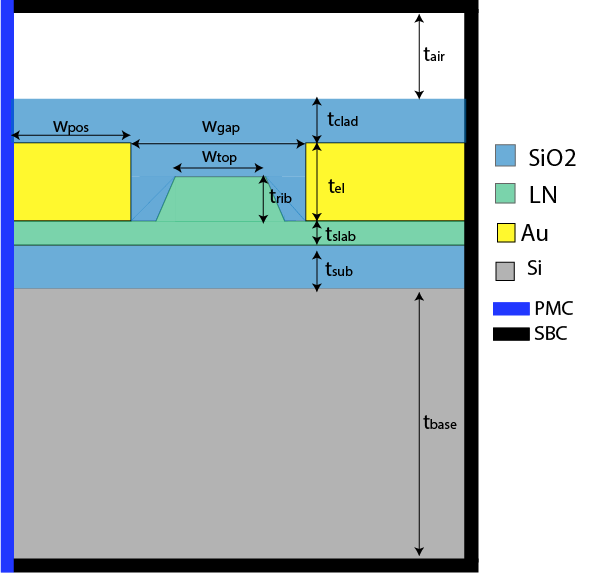
\includegraphics[width=0.85\linewidth]{simulation geometry.png} % replace with your image
    			\caption{Simulated Geometry}
    		\label{fig:microwave2D_wang-et-al}
		\end{minipage}%
\hfill
    \begin{minipage}{0.55\textwidth}
        \centering
        \begin{tabular}{|c|c|}
            \hline
            Property Name & Value  \\ \hline
            Air Thickness $(t_{air})$ & 10 $\mu m $  \\ \hline
            Cladding Thickness $(t_{clad})$ & 0.8 $\mu m $   \\ \hline
            Electrode Thickness $(t_{el})$ & 1.1 $\mu m $   \\ \hline
            Rib Thickness $(t_{rib})$ & 0.3 $\mu m $   \\ \hline
            Slab Thickness $(t_{slab})$ & 0.3 $\mu m $   \\ \hline
            Substrate Thickness $(t_{sub})$ & 4.7 $\mu m $  \\ \hline
            Base Thickness $(t_{base})$ & 500 $\mu m $    \\ \hline
            Positive Electrode Width $(w_{pos})$ & 4 $\mu m $  \\ \hline
            Gap $(w_{gap})$ & 9.895 $\mu m $    \\ \hline
            Rib Top Width $(w_{top})$ & 0.8 $\mu m $    \\ \hline
            $V_\pi L$ & 2.4115V    \\ \hline
        \end{tabular}
        \captionof{table}{Properties of simulated structure \cite{14}}
        \label{table:wang-et-al}
    \end{minipage}
\end{figure}
   

    In the Table \ref{table:wang-et-al}, calculated $V_{\pi}.L$ value and corresponding dimensions are given. In this work, $V_\pi L$ product is calculated via Equation (\ref{eq:vpiL-calculation_on_matlab}) on COMSOL-MATLAB Livelink interface. $V_{\pi}L$ value given in the paper \cite{14} is 2.3V. The error in calculation of $V_{\pi}L$ value is 4.8\%. In the Figure \ref{fig:microwave2D_wang-et-al}, the general simulation details are seen. Blue line on the left edge of geometry was included to mirror the structure to the left and PMC stands for perfect magnetic conductor. Remaining edges indicated with black lines demonstrate scattering boundary condition (SBC) to obtain results similar to real world behavior. That boundary is transparent for scattered waves.
    
    
   	
	
	\begin{figure}[h!]
        \centering
        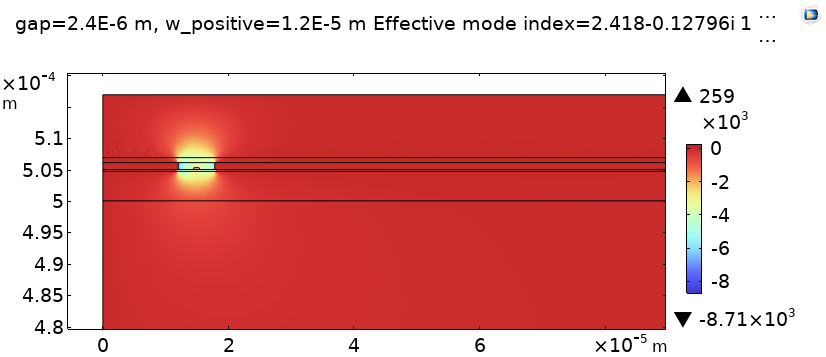
\includegraphics[width=0.8\linewidth]{field_overview_wpos_12um_gap_2.45um.png}
        \caption{Microwave field distribution in the CPW slot at 50GHz}
        \label{fig:cpw field distribution}
    \end{figure}
    
	In Figure \ref{fig:cpw field distribution}, one of the simulation result of microwave electric field's x-component is seen indicating the field confinement area. 	
	
	The aim at this point is to pinpoint microwave mode index and characteristic impedance of the transmission line. In Section \ref{sec:coplanar_waveguide}, the parameters which determines mode index characteristics and characteristic impedance are given. In this simulation, positive electrode width ($\omega _{pos}$) and gap ($\omega _{gap}$) are critical.
	

	Dynamic relation between $w_{pos}$, $w_{gap}$ and effective mode index is seen in Figure \ref{fig:index-change_colormap}. Based on this data and Equation (\ref{eq:neff_to_ng}), microwave group index is calculated. The data is seen in Figure \ref{fig:index-change_colormap} is obtained at 50GHz and additional simulation had been carried out at 55Ghz so that group index value is derived. 	
	
	\begin{equation}
		n_{el} = n_{eff} + f_{el} \pdv{n_{eff}}{f_{el}}
		\label{eq:neff_to_ng}
	\end{equation}   
	
	\newpage    
    % ------------------
	%\begin{figure}[h!]
    %    \centering
    %    \includegraphics[width=0.65\linewidth]{effective index colormap.png}
    %    \caption{Microwave mode index change color map based on $w_{gap}$ and $w_{pos}$ }
    %    \label{fig:index-change_colormap}
    %\end{figure}    
    % ------------------
	Increase of positive electrode width triggers an increase at the real part of microwave mode index and the increase of gap between electrodes causes decrease of microwave group index in Figure \ref{fig:index-change_colormap}. 
	
	 %\begin{figure}[h!]
     %	\begin{minipage}{0.5\textwidth}
     %			\centering
    %		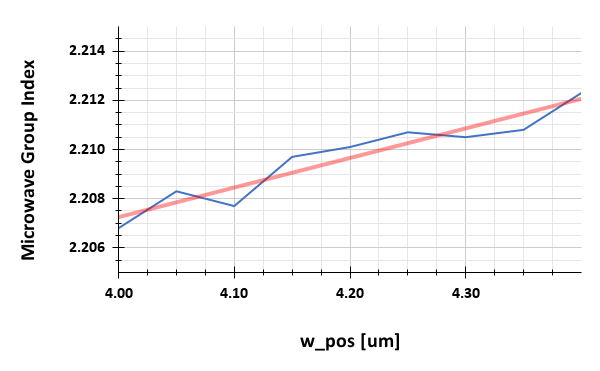
\includegraphics[width=0.85\linewidth]{microwave_group_index_w-pos.png}
    %			\caption{Simulated Geometry}
    %		\label{fig:ng_wpos}
	%	\end{minipage}%
	%	\hfill
    %	\begin{minipage}{0.55\textwidth}
    %    	\centering
     %   	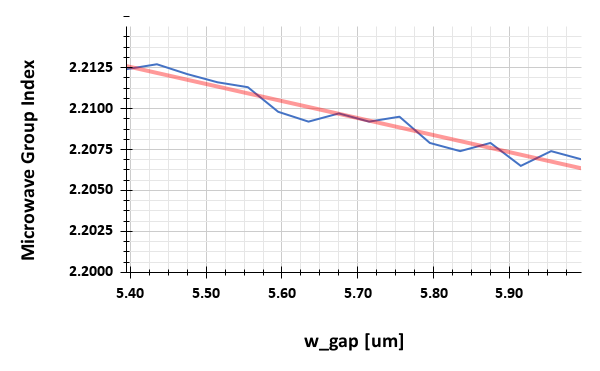
\includegraphics[width=0.85\linewidth]{microwave_group_index_gap.png}
      %  	\caption{Properties of simulated structure \cite{14}}
       % 	\label{fig:ng_wgap}
    	%\end{minipage}
	%\end{figure}
	
    As for the characteristic impedance of the line, calculations are based on the formula 
    
    \begin{equation}
    	Z_0 = \frac{V_o^2}{2P_{z-avg}}
    	\label{eq:experimental_char_imp}
    \end{equation}
    
    where $V_o$ is derived by the line integral of $E_x$ field along the gap between metal electrodes and $P_{z-avg}$ is time-average power integral into the geometry. Surface integral area is on the whole surface except metals electrodes. 
    
    For characteristic impedance calculation in Equation (\ref{eq:experimental_char_imp}), power term is multiplied by 2 and this indicates double the power obtained from simulations geometry given in Figure \ref{fig:microwave2D_wang-et-al}. In order to reduce simulation complexity, the geometry is divided by 2 and this halves the surface area which power integral is taken.
	% ------------------
    %\begin{figure}[h!]
    %    \centering
    %    \includegraphics[width=0.65\linewidth]{characteristic impedance colormap.png}
    %    \caption{Characteristic impedance change color map based on $w_{gap}$ and $w_{pos}$ }
    %    \label{fig:impedance-change_colormap}
    %\end{figure}
    % ------------------
    As the distance between two electrodes increases, per-unit-length-capacitance of the transmission line decreases.  Decrease of capacitance will lead to larger characteristic impedance as it is seen in Equation (\ref{eq:characteristic_impedance}). 
    
\subsubsection{Frequency Dependence CPW Parameters And Effects On Modulation Bandwidth}
    
	Frequency dependence of the two critical parameters are simulated. In Figure \ref{fig:ng_freq} and \ref{fig:Z0_freq} indicate the reason of band limitation on the response of waveguide-based electro-optic modulators. Eventually, the aim is having a index matching and impedance matching for larger frequency range. 
	
    % ------------------
	%\begin{figure}[h!]
    % 	\begin{minipage}{0.5\textwidth}
    % 			\centering
    %		\includegraphics[width=1\linewidth]{Microwave Group Index As A Function Of Frequency.png}
    %			\caption{Microwave group index \\ change depending on frequency}
    %		\label{fig:ng_freq}
	%	\end{minipage}%
	%	\hfill
    %	\begin{minipage}{0.5\textwidth}
    %    	\centering
    %    	\includegraphics[width=1\linewidth]{characteristic_impedance_vs_frequency_change.png}
    %    	\caption{Characteristic impedance change depending on frequency}
    %   	\label{fig:Z0_freq}
    %	\end{minipage}
	%\end{figure}    
	% ------------------
	
	In Figure \ref{fig:modulation_index_1}, bandwidth of non-optimized modulator is limited to 36GHz. 
    
	\begin{figure}[h!]
		\centering
        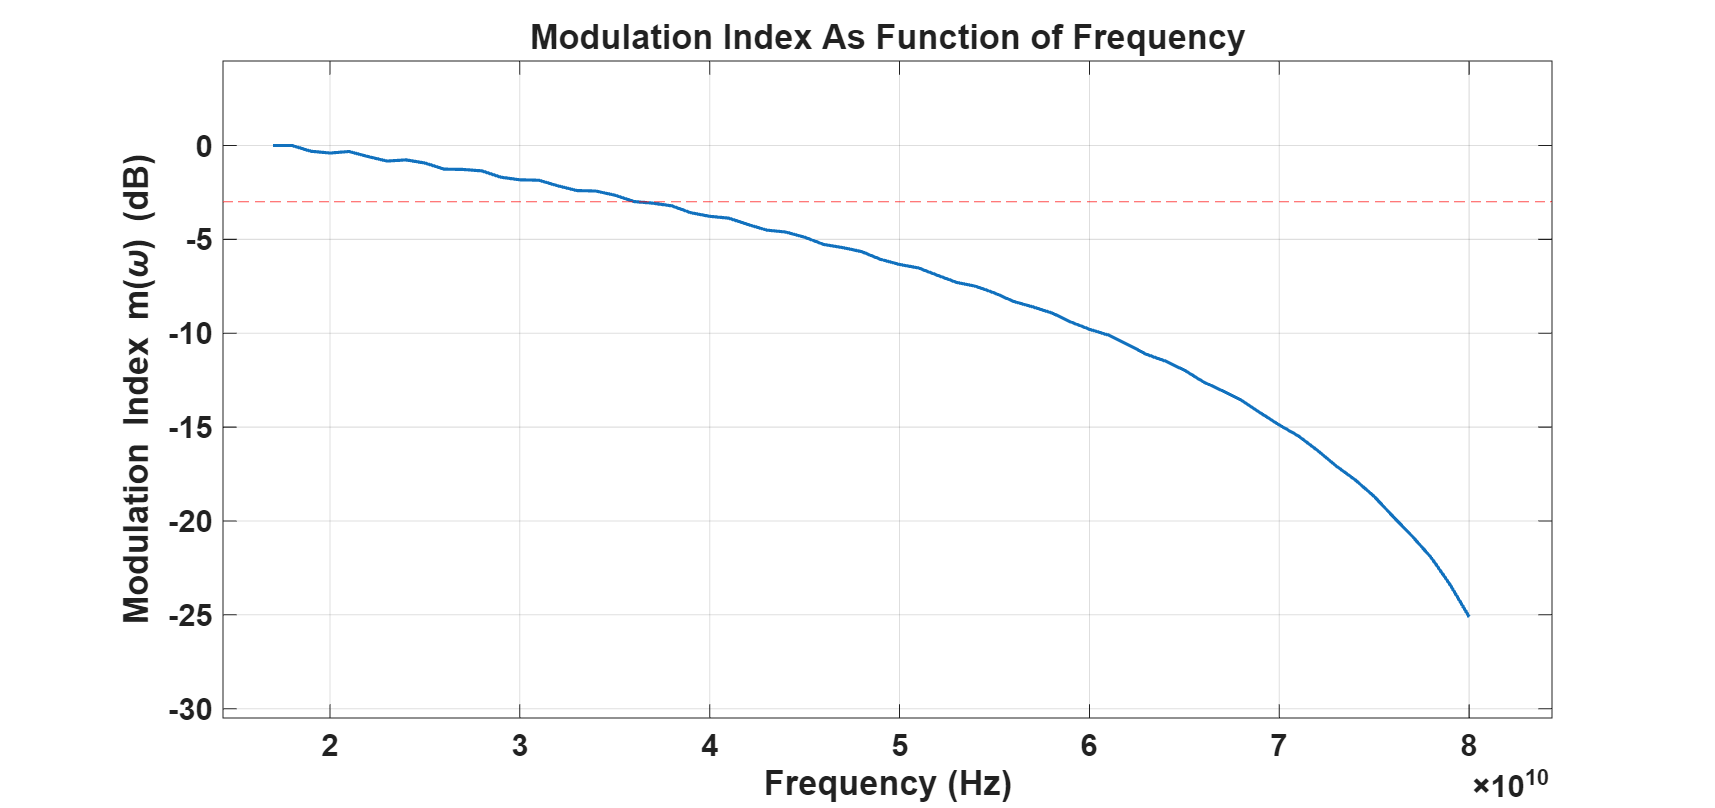
\includegraphics[width=0.9\linewidth]{modulation_index_vs_freq_15-80ghz_1ghz_step.png}
        \caption{Modulation index of the modulator geometry given in Figure \ref{fig:microwave2D_wang-et-al}. Calculation is based on the formula as in Equation (\ref{eq:eo-response})}
        \label{fig:modulation_index_1}
	\end{figure}	    
    
\subsubsection{T-Sections}
  	

   
    
    


    
\chapter{DISCUSSION}
	
    

    \subsection{Future Work}
       


\chapter{APPENDICES}

\subsection{Telegrapher's Equation}

	\begin{figure}[h]
        \centering
        \begin{circuitikz}
            \draw (0,0) to [american resistor = $R\Delta z$ ] (2,0); 
            \draw (2,0) to [american inductor = $L\Delta z$] (4,0);
            \draw (4,0) to [capacitor = $C\Delta z$ ] (4,-2);
            \draw (6,0) to [resistor = $G\Delta z$ ] (6,-2);
            \node[anchor=east] at (0,0) {\small +};
            \node[anchor=west] at (8,0) {\small +};
            \node[anchor=center] at (0,-1) {\small V(z{,}t)};	
            \node[anchor=west] at (8,-1) {\small V(z$+\Delta$ z{,}t)};
            \node[anchor=east] at (0,-2) {\small -};
            \node[anchor=west] at (8,-2) {\small -};	 
            \draw (6,0) to [short] (8,0);
            \draw (4,0) to [short] (6,0);
            \draw (0,-2) to [short] (8,-2);
        \end{circuitikz}
        \caption{Unit length model of a general transmission line}
        \label{fig:lumped_model_of_transmission_line}
    \end{figure}

	\begin{equation}
		v(z,t) - R' \Delta z \, i(z,t) - L' \Delta z \, \frac{\partial i(z,t)}{\partial t} - v(z+\Delta z, t) = 0.
	\end{equation}
	
	\begin{equation}
		- \left[ \frac{v(z+\Delta z, t) - v(z,t)}{\Delta z} \right] = R' i(z,t) + L' \frac{\partial i(z,t)}{\partial t}.
	\end{equation}
	
	
	\begin{equation}
	- \frac{\partial v(z,t)}{\partial z} 
= R' i(z,t) + L' \frac{\partial i(z,t)}{\partial t}.
	\end{equation}
	
	\begin{equation}
	- \frac{\partial v(z,t)}{\partial z} 
= R' i(z,t) + L' \frac{\partial i(z,t)}{\partial t}.
	\end{equation}
	
	\begin{equation}
i(z,t) - G' \Delta z \, v(z+\Delta z, t) 
- C' \Delta z \, \frac{\partial v(z+\Delta z, t)}{\partial t} 
- i(z+\Delta z, t) = 0.
	\end{equation}
	
	\begin{equation}
- \frac{\partial i(z,t)}{\partial z} 
= G' v(z,t) + C' \frac{\partial v(z,t)}{\partial t}.
	\end{equation}
	
	\begin{equation}
v(z,t) = \Re \big[ \tilde{V}(z) e^{j\omega t} \big], \qquad
i(z,t) = \Re \big[ \tilde{I}(z) e^{j\omega t} \big],
	\end{equation}

	\begin{equation}
- \frac{d \tilde{V}(z)}{dz} = \big(R' + j \omega L'\big)\, \tilde{I}(z),
\qquad
- \frac{d \tilde{I}(z)}{dz} = \big(G' + j \omega C'\big)\, \tilde{V}(z).
	\end{equation}

	\begin{equation}
\frac{d^{2} \tilde{V}(z)}{dz^{2}} - \gamma^{2} \tilde{V}(z) = 0,
\qquad \text{(wave equation for $\tilde{V}(z)$)} 
	\end{equation}
	
	\begin{equation}
\frac{d^{2} \tilde{I}(z)}{dz^{2}} - \gamma^{2} \tilde{I}(z) = 0,
\qquad \text{(wave equation for $\tilde{I}(z)$)}
	\end{equation}
	

\begin{thebibliography}{30}
		\bibitem{1} Di Zhu, Linbo Shao, Mengjie Yu, Rebecca Cheng, Boris Desiatov, C. J. Xin, Yaowen Hu, Jeffrey Holzgrafe, Soumya Ghosh, Amirhassan Shams-Ansari, Eric Puma, Neil Sinclair, Christian Reimer, Mian Zhang, and Marko Lončar, "Integrated photonics on thin-film lithium niobate," Adv. Opt. Photon. 13, 242-352 (2021)

        \bibitem{2} Yariv, Amnon, and Pochi Yeh. 2007. Photonics: Optical Electronics in Modern Communications (version Public Access - front matter, author index, subject index). Oxford, UK: Oxford University Press.

        \bibitem{3} Ling Liao, Dean Samara-Rubio, Michael Morse, Ansheng Liu, Dexter Hodge, Doron Rubin, Ulrich D. Keil, and Thorkild Franck, "High speed silicon Mach-Zehnder modulator," Opt. Express 13, 3129-3135 (2005)

        \bibitem{4} M. Qasymeh, M. Cada and S. A. Ponomarenko, "Quadratic Electro-Optic Kerr Effect: Applications to Photonic Devices," in IEEE Journal of Quantum Electronics, vol. 44, no. 8, pp. 740-746, Aug. 2008, doi: 10.1109/JQE.2008.924430.

        \bibitem{5} W. -T. Huang et al., "Emerging Modulator Technologies in Silicon Photonics," in IEEE Nanotechnology Magazine, doi: 10.1109/MNANO.2025.3551177.

        \bibitem{6} B. Jalali and S. Fathpour, "Silicon Photonics," in Journal of Lightwave Technology, vol. 24, no. 12, pp. 4600-4615, Dec. 2006, doi: 10.1109/JLT.2006.885782.

        \bibitem{7} Smit, Meint, Kevin Williams, and Jos Van Der Tol. "Past, present, and future of InP-based photonic integration." Apl Photonics 4.5 (2019).

        \bibitem{8} N. Courjal et al., ‘Lithium Niobate Optical Waveguides and Microwaveguides’, Emerging Waveguide Technology. InTech, Aug. 01, 2018. doi: 10.5772/intechopen.76798.

        \bibitem{9} Terrasanta, Giulio, et al. "Photonic Integrated Circuits for Optical Satellite Links: A Review of the Technology Status and Space Effects." International Journal of Satellite Communications and Networking (2025).

        \bibitem{10} Robert W. Boyd, "Nonlinear Optics", 4th Edition, 2020, Academic Press, ISBN: 978-0-12-811002-7

        \bibitem{11} Frits Zernike, John E. Midwinter, "Applied Nonlinear Optics", 1973 Dover Publications, New York.

        \bibitem{12} Inder Bahl, Maurizio Bozzi, Ramesh Garg, "Microstrip Lines and Slotlines", Third Edition , Artech, 2013.

        \bibitem{13} Yanting Guo, Lianyan Li, Yunshan Zhang, Shiyuan Sun, Qihong Quan, and Yuechun Shi, "Equivalent circuit model of the traveling wave electrode for lithium niobate thin film Mach–Zehnder modulators," Appl. Opt. 63, 617-623 (2024)

        \bibitem{14} Wang, C., Zhang, M., Chen, X. et al. Integrated lithium niobate electro-optic modulators operating at CMOS-compatible voltages. Nature 562, 101–104 (2018)

        \bibitem{15} Cheng Wang, Mian Zhang, Brian Stern, Michal Lipson, and Marko Lončar, "Nanophotonic lithium niobate electro-optic modulators," Opt. Express 26, 1547-1555 (2018)

        \bibitem{16} Ghione G. Semiconductor Devices for High-Speed Optoelectronics. Cambridge University Press; 2009.

        \bibitem{17} J. P. Salvestrini, L. Guilbert, M. Fontana, M. Abarkan and S. Gille, "Analysis and Control of the DC Drift in LiNbO3 Based Mach–Zehnder Modulators," in Journal of Lightwave Technology, vol. 29, no. 10, pp. 1522-1534, May15, 2011.

        \bibitem{18} Shihao Sun, Mingbo He, Mengyue Xu, Shengqian Gao, Ziyan Chen, Xian Zhang, Ziliang Ruan, Xiong Wu, Lidan Zhou, Lin Liu, Chao Lu, Changjian Guo, Liu Liu, Siyuan Yu, and Xinlun Cai, "Bias-drift-free Mach–Zehnder modulators based on a heterogeneous silicon and lithium niobate platform," Photon. Res. 8, 1958-1963, 2020.

        \bibitem{19} Prashanta Kharel, Christian Reimer, Kevin Luke, Lingyan He, and Mian Zhang, "Breaking voltage–bandwidth limits in integrated lithium niobate modulators using micro-structured electrodes," Optica 8, 357-363 (2021).

        \bibitem{20} Q. He, J. Wang, C. Zeng, G. He and X. Xu, "Analysis and Design of High-Accuracy Driving Circuit for Wideband Phase Modulators," in IEEE Instrumentation \& Measurement Magazine, vol. 27, no. 4, pp. 76-82, June 2024.

        \bibitem{21} Mian Zhang, Cheng Wang, Prashanta Kharel, Di Zhu, and Marko Lončar, "Integrated lithium niobate electro-optic modulators: when performance meets scalability," Optica 8, 652-667 (2021) 
	
	
		\bibitem{22}  "Antenna-coupled integrated millimeterwave modulators and resonant electro-optic frequency combs", arXiv, \textit{https://arxiv.org/html/2505.04585v1}, (2025)
		
		\bibitem{23} L. Yi, Y. Li and T. Nagatsuma, "Photonic Radar for 3D Imaging: From Millimeter to Terahertz Waves," in IEEE Journal of Selected Topics in Quantum Electronics, vol. 29, no. 5: Terahertz Photonics, pp. 1-14, Sept.-Oct. 2023
		
		\bibitem{24} Z. Yu et al., "120 GHz Sub-2 V Thin-Film Lithium Niobate Modulators on Silicon Substrate Using Thick Capacitively Loaded Slow Wave Electrodes," in IEEE Photonics Journal, vol. 16, no. 6, pp. 1-5, Dec. 2024
		
		\bibitem{25} Meng, Xiangyu, et al. "Thin‐film lithium niobate modulators with ultra‐high modulation efficiency." Laser \& Photonics Reviews 19.1 (2025)		
		
		\bibitem{26} Gongcheng Yue, Hongzhi Yang, Ziyue Zhang, Ting Hao, Lin Xiao, and Yang Li, "Dual-layer capacitance-loaded thin-film lithium niobate electro-optic modulator with high modulation efficiency," Opt. Express 32, 23161-23170 (2024)
		
		\bibitem{27} Liu, Hao, et al. "Ultra-High-Efficiency Dual-Band Thin-Film Lithium Niobate Modulator Incorporating Low-k Underfill with 220 GHz Extrapolated Bandwidth for 390 Gbit/s PAM8 Transmission." arXiv preprint arXiv:2411.15037 (2024)
		
		\bibitem{28} Gengxin Chen, Kaixuan Chen, Ranfeng Gan, Ziliang Ruan, Zong Wang, Pucheng Huang, Chao Lu, Alan Pak Tao Lau, Daoxin Dai, Changjian Guo, Liu Liu; High performance thin-film lithium niobate modulator on a silicon substrate using periodic capacitively loaded traveling-wave electrode. APL Photonics 1 February 2022
		
		\bibitem{29} Hu, Y., Zhu, D., Lu, S. et al. Integrated electro-optics on thin-film lithium niobate. Nat Rev Phys 7, 237–254 (2025).
		\end{thebibliography}

\end{document}
